
%%%%%%%%%%%%%%%%%%%%%%% file typeinst.tex %%%%%%%%%%%%%%%%%%%%%%%%%
%
% This is the LaTeX source for the instructions to authors using
% the LaTeX document class 'llncs.cls' for contributions to
% the Lecture Notes in Computer Sciences series.
% http://www.springer.com/lncs       Springer Heidelberg 2006/05/04
%
% It may be used as a template for your own input - copy it
% to a new file with a new name and use it as the basis
% for your article.
%
% NB: the document class 'llncs' has its own and detailed documentation, see
% ftp://ftp.springer.de/data/pubftp/pub/tex/latex/llncs/latex2e/llncsdoc.pdf
%
%%%%%%%%%%%%%%%%%%%%%%%%%%%%%%%%%%%%%%%%%%%%%%%%%%%%%%%%%%%%%%%%%%%


\documentclass[runningheads,a4paper]{llncs}

\usepackage{amsmath}
\usepackage{amssymb}
\usepackage{alltt}
\usepackage{lineno}
\setcounter{tocdepth}{3}
\usepackage{graphicx}
\usepackage[normalem]{ulem}

%%%%%%%%%%%%%%%%%%%%%%%%%%%%%%%%
% stuff added by phaller

\usepackage{fleqn}
\usepackage{math}
\usepackage{bcprules}
\usepackage{prooftree}

% commas and semicolons
\newcommand{\comma}{,\,}
\newcommand{\commadots}{\comma \ldots \comma}
\newcommand{\semi}{;\mbox{;};}
\newcommand{\semidots}{\semi \ldots \semi}

% spacing
\newcommand{\gap}{\quad\quad}
\newcommand{\biggap}{\quad\quad\quad}
\newcommand{\nextline}{\\ \\}
\newcommand{\htabwidth}{0.5cm}
\newcommand{\tabwidth}{1cm}
\newcommand{\htab}{\hspace{\htabwidth}}
\newcommand{\tab}{\hspace{\tabwidth}}
\newcommand{\linesep}{\ \hrulefill \ \smallskip}

% math stuff
\newenvironment{myproof}{{\em Proof:}}{$\Box$}
\renewenvironment{proofsketch}{{\em Proof Sketch:}}{$\Box$}
\newcommand{\Case}{{\em Case\ }}

% brackets
\newcommand{\set}[1]{\{#1\}}
\newcommand{\sbs}[1]{\lquote #1 \rquote}

% arrays
\newcommand{\ba}{\begin{array}}
\newcommand{\ea}{\end{array}}
\newcommand{\bda}{\[\ba}
\newcommand{\eda}{\ea\]}
\newcommand{\ei}{\end{array}}
\newcommand{\bcases}{\left\{\begin{array}{ll}}
\newcommand{\ecases}{\end{array}\right.}

% misc symbols
\newcommand{\dhd}{\!\!\!\!\!\rightarrow}
\newcommand{\Dhd}{\!\!\!\!\!\Rightarrow}
%\newcommand{\ts}{\,\vdash\,}
%\renewcommand{\ts}{\,\vdash\,}
\newcommand{\la}{\langle}
\newcommand{\ra}{\rangle}
\newcommand{\ie}{{\em i.e.}}
\newcommand{\eg}{{\em e.g.}}

%%%%%%%%%%%%%%%%%%%%%%%%%%%%%%%%%%%%%%%
%   Language abstraction commands     %
%%%%%%%%%%%%%%%%%%%%%%%%%%%%%%%%%%%%%%%

%% Relations
% Subtype 
\newcommand{\sub}{<:}
% Type assignment
\newcommand{\typ}{:}
% reduction
\newcommand{\reduces}{\;\rightarrow\;}
% well-formedness
\newcommand{\wf}{\;\mbox{\textbf{wf}}}

%% Operators
% Type selection
\newcommand{\tsel}{\#}
% Function type
\newcommand{\tfun}{\rightarrow}
\newcommand{\dfun}[3]{(#1\!:\!#2) \Rightarrow #3}
% Conjunction
\newcommand{\tand}{\wedge}
% Disjunction
\newcommand{\tor}{\vee}
% Singleton type suffix
\newcommand{\sing}{.\textbf{type}}

%% Syntax
% Header for typing rules
\newcommand{\judgement}[2]{{\bf #1} \hfill \fbox{#2}}
% Refinement
\newcommand{\refine}[2]{\left\{#1 \Rightarrow #2 \right\}}
% Field definitions
\newcommand{\ldefs}[1]{\left\{#1\right\}}
% Member sequences
\newcommand{\seq}[1]{\overline{#1}}
% Lambda
\newcommand{\dabs}[3]{(#1\!:\!#2)\Rightarrow #3}
\newcommand{\abs}[3]{\lambda #1\!:\!#2.#3}
% Application
\newcommand{\app}[2]{#1\;#2}
% Substitution
\newcommand{\subst}[3]{[#1/#2]#3}
% Object creation
\newcommand{\new}[3]{\textbf{val }#1 = \textbf{new }#2 ;\; #3}
%\renewcommand{\new}[3]{#1 \leftarrow #2 \,\textbf{in}\, #3}
% Field declaration
\newcommand{\Ldecl}[3]{#1 \typ #2..#3}%{#1 \operatorname{>:} #2 \operatorname{<:} #3}
\newcommand{\ldecl}[2]{#1 \typ #2}
% Top and Bottom
\newcommand{\Top}{\top}%{\textbf{Top}}
\newcommand{\Bot}{\bot}%\textbf{Bot}}
% Environment extension
\newcommand{\envplus}[1]{\uplus \{ #1 \}}
% Reduction
%\newcommand{\reduction}[4]{#1 \operatorname{|} #2 \reduces #3 \operatorname{|} #4}
\newcommand{\reduction}[6]{#1, #2, #3 \reduces #4, #5, #6}
\newcommand{\reduce}[4]{#1~|~#2 \;\longrightarrow\; #3~|~#4}
\newcommand{\reducebreak}[4]{#1, #2 \\ \;\longrightarrow\; #3, #4}

\newcommand{\sreduce}[8]{#1, #2, #3, #4 \;\longrightarrow\; #5, #6, #7, #8}
\newcommand{\sreducebreak}[8]{#1, #2, #3, #4 \\ \;\longrightarrow\; #5, #6, #7, #8}
\newcommand{\sreducestar}[8]{#1, #2, #3, #4 \;\longrightarrow^{\ast}\; #5, #6, #7, #8}

% end stuff added by phaller
%%%%%%%%%%%%%%%%%%%%%%%%%%%%%%%%

\usepackage{url}
\urldef{\mails}\path|firstname.lastname@epfl.ch|    
\newcommand{\keywords}[1]{\par\addvspace\baselineskip
\noindent\keywordname\enspace\ignorespaces#1}

\makeatletter
\newcommand{\customlabel}[2]{%
\protected@write \@auxout {}{\string \newlabel {#1}{{#2}{}}}}
\makeatother

\begin{document}

\mainmatter  % start of an individual contribution

% first the title is needed
\title{FlowPools: Lock-Free Deterministic Concurrent Dataflow Queues}

% a short form should be given in case it is too long for the running head
\titlerunning{FlowPools: Lock-Free Deterministic Concurrent Dataflow Queues}

% the name(s) of the author(s) follow(s) next
%
% NB: Chinese authors should write their first names(s) in front of
% their surnames. This ensures that the names appear correctly in
% the running heads and the author index.
%
\author{Authors}
%
% \author{Alfred Hofmann%
% \thanks{Please note that the LNCS Editorial assumes that all authors have used
% the western naming convention, with given names preceding surnames. This determines
% the structure of the names in the running heads and the author index.}%
% \and Ursula Barth\and Ingrid Haas\and Frank Holzwarth\and\\
% Anna Kramer\and Leonie Kunz\and Christine Rei\ss\and\\
% Nicole Sator\and Erika Siebert-Cole\and Peter Stra\ss er}

\authorrunning{FlowPools: Lock-Free Deterministic Concurrent Dataflow Queues}
% (feature abused for this document to repeat the title also on left hand pages)

% the affiliations are given next; don't give your e-mail address
% unless you accept that it will be published
\institute{EPFL, Switzerland\\
\mails\\
\url{http://lamp.epfl.ch}}

%
% NB: a more complex sample for affiliations and the mapping to the
% corresponding authors can be found in the file "llncs.dem"
% (search for the string "\mainmatter" where a contribution starts).
% "llncs.dem" accompanies the document class "llncs.cls".
%

% \toctitle{Lecture Notes in Computer Science}
% \tocauthor{Authors' Instructions}
\maketitle


\begin{abstract}
Implementing correct and deterministic parallel programs is challenging. Even
though concurrency constructs exist in popular programming languages to
facilitate the task of deterministic parallel programming, they're often too
low level, or do not compose well due to underlying blocking mechanisms. In
this paper, we present the design and implementation of a fundamental data
structure for composable deterministic parallel dataflow computation through
the use of functional programming abstractions. Additionally, we provide a
proof of correctness, showing that the implementation is linearizable, lock-
free, and deterministic. Finally, we provide experimental results which
compare our \emph{FlowPool} against corresponding operations on other popular
concurrent data structures, and show that in addition to offering new
capabilities, FlowPools perform XYZ-XYZ\% better than their blocking counterparts.
\keywords{dataflow, concurrent data-structure, deterministic parallelism}
\end{abstract}


\section{Introduction}

Multicore architectures have become ubiquitous-- even most mobile devices now
ship with multiple core processors. Yet parallel programming has yet to enter
the daily workflow of the mainstream developer. One significant obstacle is an
undesirable choice programmers must often face when solving a problem that
could greatly benefit from leveraging available parallelism. Either choose a
non-deterministic, but performant, data structure or programming model, or
sacrifice performance for the sake of clarity and correctness.

Programming models based on \emph{dataflow} \cite{Arvind89,CnC10} have the
potential to simplify parallel programming, since the resulting programs are
deterministic. Moreover, dataflow programs can be expressed more declaratively
than programs based on mainstream concurrency constructs, such as shared-memory 
threads and locks, as programmers are only required to specify data and
control dependencies. This allows one to reason sequentially about the
intended behavior of their program, meanwhile enabling the underlying
framework to automatically and effectively extract parallelism.

In this paper, we present the design and implementation of FlowPools, a
fundamental dataflow collections abstraction which can be used as a building
block to build larger and more complex \textit{deterministic} and parallel
dataflow programs. Our FlowPool abstraction is backed by an efficient non-
blocking data structure, which we go on to prove is lock-free.

As a result, our data structure benefits from the increased robustness
provided by lock freedom~\cite{Herlihy90}, since its operations are unaffected
by thread delays. We provide a lock freedom proof, which guarantees progress
regardless of the behavior, including the failure, of concurrent threads.

% I don't like how it says "we go on to show"
In combining lock-freedom with a functional interface, we go on to show that
FlowPools are \textit{composable}. That is, using prototypical higher-order
functions such as \verb=foreach= and \verb=aggregate=, one can concisely form
dataflow graphs, in which associated functions are executed asynchronously in
a completely non-blocking way, as elements of FlowPools in the dataflow graph
become available.

% I don't like how it says "we show"
Finally, we show that FlowPools are able to overcome practical issues, such as
out-of-memory errors, thus enabling programs based upon FlowPools to run
indefinitely. By using a \textit{builder} abstraction, instead of something
like iterators or streams (which either lead to non-determinism or require
that all elements stay in memory) we are able to garbage collect parts of the
data structure we no longer need, thus reducing memory consumption.

Our contributions are the following:
\begin{enumerate}
\item The design and implementation of parallel dataflow abstraction and
underlying data structure that is deterministic, lock-free, and composable.
\item Proofs of lock-freedom, linearizability, and determinism.
\item Detailed benchmarks comparing the performance our FlowPools against
other popular concurrent data structures.
\end{enumerate}

% === OTHER THINGS TO ADDRESS... ===
% memory stuff.
    % - programs run indefinitely $\Rightarrow$ we need to GC parts of the
    % data structure we no longer need
    % - we want to reduce heap allocation and inline the data structure as
    % much as possible $\Rightarrow$ lower memory consumption, better cache behaviour
    % and fewer GC cycles
% === ... ===

% vvvvvvv MAYBE KEEP THIS?? vvvvvvv

% This paper remedies the shortcomings of an imperative vs functional approach.
% On the one had, the main issue with imperative programs in concurrent
% environments is mutable state, and the race conditions that result from such
% situations. On the other hand, functional programming provides the guarantee
% that state can never be changed, resulting in concise and correct code, but
% which often performs poorly due to the overhead of only ever creating new
% objects and never reusing old ones, thereby increasing the pressure on the
% garbage collector. Our approach is to combine the benefits of each of these
% approaches. We provide a concise and easy-to-reason-about deterministic
% functional interface on top of an imperative but performant and provably
% correct implementation.

% ^^^^^ MAYBE KEEP THIS?? ^^^^^

% In this paper, we advocate an approach that achieves high performance and
% composability at the same time through combining high-level functional
% abstractions with an efficient non-blocking implementation.

% In this paper, we advocate a dataflow programming model to .


% Why is a deterministic programming model preferable? Reason sequentially.
% Another advantages is that data dependencies are expressed as a way to enable
% the underlying runtime system to effectively extract parallelism.

% In our model, the above point is achieved through the composability afforded
% by using functional abstractions.

% 1) How do we achieve determinism in the first place. Design of programming.
% 2) How do we make dataflow/determinism more usable in practice to build larger
% program. This is where composability comes into play. Build larger programs
% from reusable parts.

% By being able to start asynchronous computations as soon as their required
% inputs have been computed.

% The shift in recent years by processor manufacturers from single to
% multi-core architectures, academia and industry alike have conceded that
% \textit{Popular Parallel Programming} remains a formidable challenge. Even our
% cellphones are now multicore.

% the choice between performance, leading to the use of 
% non- deterministic data structures or programming models whose semantics are
% difficult to reason about, and clarity, leading clear and correct but non-
% performant code. 

% non-deterministic code hard to debug because you have all of these different
% thread interleavings that have to be taken into account when designing the
% program. whereas a deterministic program doesn't have to consider thread
% interleavings because they don't have an effect on the outcome of a result.

% While non-blocking techniques have been used for building high-performance
% concurrent data structures, they . There exist non-blocking concurrent data
% structures, but not necessarily non-blocking concurrent deterministic data
% structures.

% What can prevent composability is lock-based. 

% Something that can provide composability is functional combinators. 

% \textbf{Lock-free is better, and why.} 
% \sout{why the foreach instead of blocking?} blocking is bad in most
%    programming models (JVM, CLR, most native platforms) \cite{Herlihy90}

% Introduction and motivation for data-flow programming model.

% Data structures for the multicore age, Shavit 2011, Comm. ACM \cite{Shavit11}

% Concurrent data structures, Moir, Shavit 2008, \cite{Moir05}

% A Methodology for Implementing Highly Concurrent Data Structures, Herlihy, 1990 \cite{Herlihy90}

% \subsection{Motivation}

% \textbf{Paragraph(s) on shortcomings of typical approaches.} 
% -\sout{Plus,} iterators or streams would not be deterministic. Even if they
% are thread-safe, they have an inherent state which can lead to nondeterminism.
% - \sout{But this} leads to GC problems! We have to keep every element around
% forever. Computations can run arbitrarily long (GC point)

% \textbf{Paragraph(s) stating goals.} 
% - we want a deterministic model. we do not block in the programming model (i.e. there are no
% operations which cause blocking until a value becomes available)
% - we want a non-blocking data-structure (i.e. the operations on the
% data-structures should themselves be non-blocking)
% - programs run indefinitely $\Rightarrow$ we need to GC parts of the
% data structure we no longer need
% - we want to reduce heap allocation and inline the data structure as
% much as possible $\Rightarrow$ lower memory consumption, better cache behaviour
% and fewer GC cycles
% - composability

% We present concurrent data structure . We jointly focus on performance and
% extending the capabilities of queue-like data structures for dataflow
% computation.


\section{Model of Computation}

Pipeline-based applications are composed of a sequence
of producer/consumer stages, each one depending on the output of its
predecessor. More generally, the computation forms a directed
dependency graph in which parallelism is achieved by operations in
different nodes executing concurrently.

One design goal is to make the nodes in the dependency graph first
class values.
The advantage of this is that the programmer is able to use
nodes as procedure arguments or receive them as return values.
This allows for a better modularity and increases the
composability of the programming model.
It also provides a higher degree of flexibility -- the dependency
graph does not have to be specified at compile time, but can be
computed at runtime instead.

\textbf{Determinism}.

Throughout this paper, we follow notion of determinism introduced by the Oz
programming language \cite{RoyH2004} as \textit{declarative concurrency}; "a
concurrent program is declaratively concurrent if and only if all possible
executions either do not terminate or they all eventually reach logically
equivalent results." In this definition, non-termination also includes
exceptions that occur at runtime. Furthermore, logically equivalent results
mean that resulting data structures are in the same state. This is
convenient for the programmer-- if an exception occurs in some run of a
program, then it is guaranteed to occur in every run of the program. However,
if there are no exceptions, then the program is guaranteed to be
deterministic.

% What do we mean by determinism?
% We seek a definition of determinism that is practically
% useful, first and foremost in the sense that it makes debugging parallel
% programs easier. 
% Thus, throughout this paper, we strive to fit the definition
% of declarative concurrency from the Oz programming language \cite{RoyH2004},
% "a concurrent program is declaratively concurrent if and only if all possible
% executions either do not terminate or they all eventually reach logically
% equivalent results." In this definition, non-termination also includes
% exceptions that occur at runtime. Furthermore, logically equivalent results roughly denote
% that the data structures are in the same state. This is convenient for the
% programmer-- if an exception occurs in some run of a program, then it is
% guaranteed to occur in every run of the program. However, if there are no
% exceptions, then the program is guaranteed to be deterministic.

In this paper we describe a deterministic pool abstraction which allows
appending elements and then traversing them.
We call this data structure a \textit{single-assignment pool} or a FlowPool.
Such an abstraction may seem similar to the dataflow streams seen in Oz,
but there are some important differences.
We argue that both of these are deterministic, but our pool abstraction
does not define the order between contained elements, hence there is
no predefined traversal order.

The simplified model of computation is shown in Fig. \ref{TODO}.
The pool abstraction usually defines adding elements and retrieving
some element previously added.
This retrieval is not very useful unless it also removes the element.
In a concurrent setting such a remove is time-dependent and gives
different results depending on when it was called -- an element
present at one point might not be present later.
Such an operation would hinder determinism.
For this reason we do not provide a way to remove an element once it
has been added.
Instead, we provide a way to express what should be done with each
element of the pool -- traversal.
Finally, we allow the pool to be sealed to a certain size -- this
bounds the number of elements that can be added to the pool.

\subsection{Syntax and operations}

\smallrulenames

\begin{figure}[t]
%\figurebox{
%{\bf Syntax}\medskip

%$\ba{l@{\hspace{2mm}}|@{\hspace{2mm}}l}
%$\ba[t]{l}

$\ba[t]{l@{\hspace{2mm}}l}
t    ::=                                                           & \mbox{terms}              \\
\gap p << v                                                  & \mbox{append}           \\
\gap \texttt{create}~p                                   & \mbox{pool creation}  \\
\gap p~\texttt{foreach}~f                             & \mbox{foreach}           \\
\gap p~\texttt{seal}~n                                  & \mbox{seal}                \\
\gap \texttt{nop}                                          & \mbox{no op}              \\
\gap t_1~;~t_2                                               & \mbox{sequence}        \\
\ea$

$\ba{l@{\hspace{2mm}}|@{\hspace{2mm}}l@{\hspace{2mm}}l}
p \in \set{(vs, \sigma, cbs)~|~vs \subseteq Elem, \sigma \in \set{-1} \cup \mathbb{N}, cbs \subset Elem \Rightarrow Unit} & v \in Elem \\
f \in Elem \Rightarrow Unit & n \in \mathbb{N}
\ea$

%\ea$

%}
\caption{Syntax}\label{fig:syntax}
\end{figure}



\section{Programming Interface}
\label{sec:programming-interface}

A FlowPool can be viewed as a concurrent pool data structure, and as such has
no guarantees on ordering. In this section, we describe the semantics of a
handful of functional combinators and other basic operations defined on
FlowPools.

\textbf{Append (\texttt{<<})}. The most fundamental of all
operations of on FlowPools is the append operation. As its name suggests, it
simply takes an argument of type \texttt{Elem} and appends it to a given
FlowPool. 

% notice -- we could have a stream returned from the pool instead and
% poll the stream until the value arrives -- but this leads to blocking.

% \sout{what should be the semantics of the foreach - should it execute only
% for elements added to the flowpool after calling foreach? or} should it
% execute for all the elements ever added?
% \sout{The latter --} we want determinism, avoid races, same execution every
% time.

\textbf{Foreach and Aggregate.}
A pool containing a set of elements is of little use if the elements
cannot be manipulated in some manner.
One of the basic data structure operations is element traversal,
often provided by iterators or streams -- stateful
objects storing the current position in the data structure.
Since they can be manipulated by several threads, they allow
nondeterministic execution.

Another way to traverse the elements is to provide a higher-level
\verb=foreach= operations which takes a user-specified function and
applies it to every element.
To ensure determinism, it is called for every element that is
eventually in the FlowPool, rather than only those present
when \verb=foreach= is called.
To ensure non-blocking behaviour, it must not wait until
additional elements are added to the FlowPool.
For these reasons, the \verb=foreach= operation must execute
asynchronously and is eventually applied to every element.
Its signature is \verb+def foreach[U](f: T => U): Future[Int]+.
The return type \verb=Future[Int]= is an integer value which becomes
available once \verb=foreach= traverses all the elements added to the
pool.
It denotes the number of times the \verb=foreach= has been called.
The user-specified function return value of type \verb=U= is ignored.

The \verb=aggregate= operation aggregates the elements of the pool
together and has the following signature: \verb+def aggregate[S]+\verb+(zero: =>S)+
\verb+(cb: (S, S) => S)+ \verb+(op: (S, T) => S):+ \verb+Future[S]+,
where \verb=zero= is the initial aggregation, \verb=cb= is an
associative operator which combines several aggregations, \verb=op= is
an operator that adds an element to the aggregation, and
\verb=Future[S]= is the final aggregation of all the elements which
becomes available once all the elements have been added.
The \verb=aggregate= divides elements into subsets and applies the
aggregation operator \verb=op= to aggregate elements in each subset
starting from the \verb=zero= aggregation, and then combines
aggregations from different subsets with the \verb=cb= operator.
In essence, the first part of \verb=aggregate= defines the commutative
monoid and the functions involved must be non-side-effecting.
In contrast, the \verb=op= is guaranteed to be called only once per
each element and it can have side-effects.

While in an imperative programming model \verb=foreach= and \verb=aggregate= are
equivalent in the sense that one can be implemented in terms of the
other, in a single-assignment programming model \verb=aggregate= is more
expressive than \verb=foreach=.
The \verb=foreach= can be implemented using \verb=aggregate=, but not vice versa,
due to the absence of side-effects.

\textbf{Builders.}
The FlowPool described so far is that it must maintain a reference 
to all the elements at all times to implement the \verb=foreach=
correctly.
Since elements are never removed, the pool may grow indefinitely
and run out of memory.

In the same time appending new elements does not require a reference
to any of the existing elements.
We use this observation to factor out the \verb=<<= operation into
a different abstraction called a \verb=builder=.
A typical application starts by registering all the \verb=foreach=
operations and then releases the references to FlowPools.
In a managed environment the GC then implicitly takes care of
discarding the no longer needed objects.


\textbf{Seal.}
When the client is sure that no more elements will be added to the pool
he can disallow further appends by calling \verb=seal=.
This has the advantage of discarding the registered \verb=foreach=
operations.
More importantly, \verb=aggregate= can only complete the future
once it is certain that no more elements will be added.

A \verb=seal= which just closes the FlowPool at the moment when it
is called, however, yields a nondeterministic programming model.
Imagine a thread that attempts to seal the pool executing concurrently
with a thread that appends an element.
In one execution, the append preceeds the seal, and in the other
the append follows the seal causing an error.
To avoid nondeterminism, there has to be an agreement on the
state of the pool when it is sealed.
A convenient and sufficient way to make `seal` deterministic
is to provide the expected size.
The semantics of \verb=seal= are then such that it fails if the pool
is already sealed with a different size or the number of elements
is greater than the desired size.

\textbf{Higher-level operations.}
We now show how the basic abstractions above can be used
to build higher-level abstractions.
To begin with, in addition to a default FlowPool constructor, it is
convenient to have generators which create certain types of pools.
In a dataflow graph FlowPools created using generators
are source nodes.
As a simple example, \verb=tabulate= creates a sequence of elements
by applying a user-specified function \verb=f= to each natural number.
One can imagine more complicated generators, adding elements from a
network socket or a file.

Generator \verb=tabulate= starts by creating a FlowPool of an
arbitrary type \verb=T= and creating its builder instance.
It then starts an asynchronous computation using the \verb=future=
construct, which recursively applies \verb=f= to each number and
appends it to the builder.
Finally, the reference to the pool is returned.

\noindent
\begin{minipage}[b]{4.2 cm}
\begin{alltt}
{\scriptsize
def tabulate[T]
  (n: Int, f: Int => T)
  val p = new FlowPool[T]
  val b = p.builder
  def recurse(i: Int) \{
    b << f(i)
    if i < n recurse(i + 1)
  \}
  future \{ recurse(0) \}
  p
}
\end{alltt}
\end{minipage}\begin{minipage}[b]{4 cm}
\begin{alltt}
{\scriptsize
def map[S](f: T => S)
  val p = new FlowPool[S]
  val b = p.builder
  for (x <- this) \{
    b << f(x)
  \} map \{
    sz => b.seal(sz)
  \}
  p

}
\end{alltt}
\end{minipage}
\begin{minipage}[b]{2.5 cm}
\begin{alltt}
{\scriptsize
def foreach[U](f: T => U)
  aggregate(0)(_ + _) \{
    (acc, x) =>
    f(x)
    acc + 1
  \}




}
\end{alltt}
\end{minipage}

A typical higher-level collection operation \verb=map= is used to
map each element of a dataset to produce a new one.
This corresponds to chaining the nodes in the dataflow graph.
We implement it by traversing the elements of \verb=this= FlowPool and
appending each mapped element to the builder.
The \verb=for= loop is the syntactic sugar for calling the
\verb=foreach= method on \verb=this=.
We assume that the \verb=foreach= return value \verb=Future[Int]=
has \verb=map= and \verb=flatMap= operations, which are executed
once the future value becomes available.
The \verb=Future.map= above ensures that if the \verb=this= pool is ever
sealed, the mapped pool is sealed to the appropriate size.

As argued before, the \verb=foreach= can be expressed in terms of a
\verb=aggregate= by accumulating the number of elements and invoking the
callback \verb=f= each time.
We further show that some patterns cannot be expressed in terms of a mere
\verb=foreach=.
The \verb=filter= combinator filters out the elements for which a
specified predicate does not hold.
Appending the elements to a new pool can proceed as
before, but the seal needs to know the exact number of elements added.
The \verb=aggregate= accumulator is thus used to track the number
of added elements.

\noindent
\begin{minipage}[b]{4 cm}
\begin{alltt}
{\scriptsize
def filter
  (pred: T => Boolean)
  val p = new FlowPool[T]
  val b = p.builder
  aggregate(0)(_ + _) \{
    (acc, x) => if pred(x) \{
      b << x
      1
    \} else 0
  \} map \{ sz => b.seal(sz) \}
  p



}
\end{alltt}
\end{minipage}\begin{minipage}[b]{4 cm}
\begin{alltt}
{\scriptsize
def flatMap[S]
  (f: T => FlowPool[S])
  val p = new FlowPool[S]
  val b = p.builder
  aggregate(future(0))(add) \{
    (af, x) =>
    val sf = for (y <- f(x))
      b << y
    add(af, sf)
  \} map \{ sz => b.seal(sz) \}
  p

def add(f: Future[Int], g: Future[Int]) =
  for (a <- f; b <- g) yield a + b
}
\end{alltt}
\end{minipage}
\begin{minipage}[b]{4 cm}
\begin{alltt}
{\scriptsize
def union[T]
  (that: FlowPool[T])
  val p = new FlowPool[T]
  val b = p.builder
  val f = for (x <- this) b << x
  val g = for (y <- that) b << y
  for (s1 <- f; s2 <- g)
    b.seal(s1 + s2)
  p





}
\end{alltt}
\end{minipage}

The \verb=flatMap= operation retrieves a pool for each element of
\verb=this= pool and adds its elements to the resulting pool.
Given two FlowPools, it can be used to generate the cartesian product
of their elements.
The implementation is similar to that of the \verb=filter=,
but we reduce the size on the future values of the sizes, because each
intermediate pool may not yet be sealed.
%Implementing this operation is sufficient to show that a FlowPool is
%a monad.
The \verb=union= operation produces a new pool which has elements of
both pool \verb=q= and pool \verb=r=.

The last two operations correspond to joining nodes in the dataflow
graph.
Note that if we could somehow merge the two different \verb=foreach=
loops to implement the third join type \verb=zip=, we would
yield a nondeterministic operation.
The programming model does not allow us to do so, however.
The \verb=zip= is more suited for data structures with deterministic ordering,
such as Oz streams -- which would in turn have a nondeterministic \verb=union=.



\begin{figure}[t]

\centering

\begin{minipage}[b]{4.5 cm}
\begin{alltt}
{\scriptsize
type Terminal \{
  sealed: Int
  callbacks: List[Elem => Unit]
\}

type Elem
}
\end{alltt}
\end{minipage}
\begin{minipage}[b]{3.5 cm}
\begin{alltt}
{\scriptsize
type Block \{
  array: Array[Elem]
  next: Block
  index: Int
  blockindex: Int
\}
}
\end{alltt}
\end{minipage}
\begin{minipage}[b]{4 cm}
\begin{alltt}
{\scriptsize
type FlowPool \{
  start: Block
  current: Block
\}
LASTELEMPOS = BLOCKSIZE - 2
NOSEAL = -1
}
\end{alltt}
\end{minipage}

\caption{FlowPool data-types}
\label{f-datatypes}
\end{figure}

\setlength\linenumbersep{2pt}


\begin{figure}

\centering

\begin{minipage}[b]{6 cm}
\begin{alltt}
{\scriptsize
{\internallinenumbers{def create()
  new FlowPool \{
    start = createBlock(0)
    current = start
  \}

def createBlock(bidx: Int)
  new Block \{
    array = new Array(BLOCKSIZE)
    index = 0
    blockindex = bidx
    next = null
  \}

def append(elem: Elem)
  b = READ(current) {\customlabel{read_block}{\LineNumber}}
  idx = READ(b.index) {\customlabel{read_index}{\LineNumber}}
  nexto = READ(b.array(idx + 1)) {\customlabel{read_next}{\LineNumber}}
  curo = READ(b.array(idx)) {\customlabel{read_current}{\LineNumber}}
  if check(b, idx, curo) \{
    if CAS(b.array(idx + 1), nexto, curo) \{ {\customlabel{cas_propagate}{\LineNumber}}
      if CAS(b.array(idx), curo, elem) \{ {\customlabel{cas_append}{\LineNumber}}
        WRITE(b.index, idx + 1) {\customlabel{write_append}{\LineNumber}}
        invokeCallbacks(elem, curo)
      \} else append(elem)
    \} else append(elem)
  \} else \{
    advance()
    append(elem)
  \}

def check(b: Block, idx: Int, curo: Object)
  if idx > LASTELEMPOS return false
  else curo match \{
    elem: Elem =>
      return false
    term: Terminal =>
      if term.sealed = NOSEAL return true
      else \{
        if totalElems(b, idx) < term.sealed
          return true
        else error("sealed")
      \}
    null =>
      error("unreachable")
  \}

def advance()
  b = READ(current)
  idx = READ(b.index)
  if idx > LASTELEMPOS
    expand(b, b.array(idx))
  else \{
    obj = READ(b.array(idx))
    if obj is Elem WRITE(b.index, idx + 1) {\customlabel{write_advance}{\LineNumber}}
  \}

def expand(b: Block, t: Terminal)
  nb = READ(b.next)
  if nb is null \{
    nb = createBlock(b.blockindex + 1)
    nb.array(0) = t
    if CAS(b.next, null, nb) {\customlabel{cas_expand}{\LineNumber}}
      expand(b, t)
  \} else \{
    CAS(current, b, nb) {\customlabel{cas_block}{\LineNumber}}
  \}
}}}
\end{alltt}
\end{minipage}
\begin{minipage}[b]{6 cm}
\begin{alltt}
{\scriptsize
{\internallinenumbers{def totalElems(b: Block, idx: Int)
  return b.blockindex * (BLOCKSIZE - 1) + idx

def invokeCallbacks(e: Elem, term: Terminal)
  for (f <- term.callbacks) future \{
    f(e)
  \}

def seal(size: Int)
  b = READ(current)
  idx = READ(b.index)
  if idx <= LASTELEMPOS \{
    curo = READ(b.array(idx)) {\customlabel{read_seal}{\LineNumber}}
    curo match \{
      term: Terminal =>
        if \(\lnot\)tryWriteSeal(term, b, idx, size)
          seal(size)
      elem: Elem =>
        WRITE(b.index, idx + 1) {\customlabel{write_seal}{\LineNumber}}
        seal(size)
      null =>
        error("unreachable")
    \}
  \} else \{
    expand(b, b.array(idx))
    seal(size)
  \}

def tryWriteSeal(term: Terminal, b: Block,
  idx: Int, size: Int)
  val total = totalElems(b, idx)
  if total > size error("too many elements")
  if term.sealed = NOSEAL \{
    nterm = new Terminal \{
      sealed = size
      callbacks = term.callbacks
    \}
    return CAS(b.array(idx), term, nterm) {\customlabel{cas_seal}{\LineNumber}}
  \} else if term.sealed \(\neq\) size \{
    error("already sealed with different size")
  \} else return true

def foreach(f: Elem => Unit)
  future \{
    asyncFor(f, start, 0)
  \}

def asyncFor(f: Elem => Unit, b: Block, idx: Int)
  if idx <= LASTELEMPOS \{
    obj = READ(b.array(idx)) {\customlabel{read_callback}{\LineNumber}}
    obj match \{
      term: Terminal =>
        nterm = new Terminal \{
          sealed = term.sealed
          callbacks = f \(\cup\) term.callbacks
        \}
        if \(\lnot\)CAS(b.array(idx), term, nterm) {\customlabel{cas_foreach}{\LineNumber}}
          asyncFor(f, b, idx) {\customlabel{cas_callback}{\LineNumber}}
      elem: Elem =>
        f(elem) {\customlabel{call_callback}{\LineNumber}}
        asyncFor(f, b, idx + 1)
      null =>
        error("unreachable")
    \}
  \} else \{
    expand(b, b.array(idx))
    asyncFor(f, b.next, 0)
  \}
}}}
\end{alltt}
\end{minipage}

\caption{FlowPool operations pseudocode}
\label{f-pseudo}
\end{figure}

\section{Implementation}

We now describe the FlowPool and its basic operations.
In doing so, we omit the details not relevant to the
algorithm\footnote{Specifically the builder abstraction and the \texttt{aggregate}
operation. The \texttt{aggregate} can be implemented using \texttt{foreach}
with a side-effecting accumulator.}
and focus on a high-level description of a non-blocking
data structure.
One straightforward way to implement a growing pool is to use a linked
list of nodes that wrap elements.
As we are concerned about the memory footprint and cache-locality, we
store the elements into arrays instead, which we call blocks.
Whenever a block becomes full, a new block is allocated and the
previous block is made to point to the \verb=next= block.
This way, most writes amount to a simple array-write, while allocation
occurs only occasionally.
Each block contains a hint \verb=index= to the first free entry in
the array, i.e. one that does not contain an element.
An \verb=index= is a hint, since it may actually reference an earlier index.
The FlowPool maintains a reference to the first block called
\verb=start=.
It also maintains a hint to the last block in the chain of blocks,
called \verb=current=.
This reference may not always be up to date, but it always points
to some block in the chain.

Each FlowPool is associated with a list of callbacks which have
to be called in the future as new elements are added.
Each FlowPool can be in a sealed state, meaning there is a bound on
the number of elements it stores.
This information is stored as a \verb=Terminal= value in the first
free entry of the array.
At all times we maintain the invariant that the array in each block
starts with a sequence of elements, followed by a \verb=Terminal=
delimiter. From a higher-level perspective, appending an element
starts by copying the \verb=Terminal= value to the next entry and then
overwriting the current entry with the element being appended.

The \verb=append= operation starts by reading the \verb=current= block
and the \verb=index= of the free position.
It then reads the
\verb=nexto= after the first free entry, followed by a read of the
\verb=curo= at the free entry.
The \verb=check= procedure checks the bounds conditions, whether the
FlowPool was already sealed or if the current array entry contains an
element.
In either of these events, the \verb=current= and \verb=index= values
need to be set -- this is done in the \verb=advance= procedure.
We call this the \textbf{slow path} of the \verb=append= method.
Notice that there are several causes that trigger the slow path.
If some other thread completes the \verb=append= method but is
preempted before updating the value of the hint \verb=index=, then the
\verb=curo= will have the type \verb=Elem=.
The same happens if a preempted thread updates the value of the
hint \verb=index= after additional elements have been added,
via unconditional write in line \ref{write_append}.
Finally, reaching an end of block triggers the slow path.

Otherwise, the operation executes the \textbf{fast path} and appends
an element.
It first copies the \verb=Terminal= value to the next entry with a CAS
instruction in line \ref{cas_propagate}, with \verb=nexto= being the
expected value. If it fails (e.g. due to a concurrent CAS), the append
operation is restarted.
Otherwise, it proceeds by writing the element to the current entry with
a CAS in line \ref{cas_append}, the expected value being
\verb=curo=.
On success it updates the \verb=b.index= value and invokes all
the callbacks (present when the element was added) with
the \verb=future= construct.
In the implementation we do not schedule an asynchronous
computation for each element.
Instead, the callback invocations are batched to avoid the schedulling overhead
-- the array is scanned for new elements
until there are no more left.

Interestingly, inverting the order of the reads in lines
\ref{read_next} and \ref{read_current} would cause a race in which a
thread could overwrite a \verb=Terminal= value with some older
\verb=Terminal= value if some other thread appended an element in between.

The \verb=seal= operation continuously increases the \verb=index= in the block
until it finds the first free entry. It then tries to replace the \verb=Terminal=
value there with a new \verb=Terminal= value which has the seal size set.
An error occurs if a different seal size is set already. The \verb=foreach=
operation works in a similar way, but is executed asynchronously. Unlike
\verb=seal=, it starts from the first element in the pool and calls the
callback for each element until it finds the first free entry.
It then replaces the \verb=Terminal= value with a new \verb=Terminal=
value with the additional callback. From that point on the \verb=append=
method is responsible for scheduling that callback for subsequently added elements.
Note that all three operations call \verb=expand= to add an additional
block once the current block is empty, to ensure lock-freedom.

\textbf{Multi-Lane FlowPools.}
Using a single block sequence (i.e. lane) to implement a FlowPool
doesn't fully take advantage of the lack of ordering guarantees and --
as elements are inserted in sequence -- may cause slowdowns due to
collisions when multiple concurrent writers are present. Multi-Lane
FlowPools solve this limitation by having a lane for each CPU, where
each lane is following the same implementation as for a normal
FlowPool.

This has several implications:
\begin{itemize}
\item CAS failures during insertion are to a high extent avoided.
\item Less memory contetion due to ``private'' blocks for each
  processor.
\item \verb=seal= needs to be globally synchronized in a non-blocking
  fashion.
\item Callbacks for \verb=aggregate= have to be added to each lane
  individually and aggregated once all of them have completed.
\end{itemize}

In practice, a hash on the ID of the inserting thread has to be used
instead of the CPU index, as such information is currently not
available through the Java framework. Also note that the remaining
slots resulting from a \verb=seal= have to be split up amongst the
lanes and a writer might switch lanes if his lane is full (and hence
CAS failures may happen).

You find an evaluation of the performance of Multi-Lane FlowPools in
section~\ref{sec:evaluation}.

\section{Correctness}

We give an outline of the correctness proof here. More formal
definitions, complete set of lemmas and proofs can be found in the
appendix.

We define the notion of an abstract pool $\mathbb{A} = (elems,
callbacks, seal)$ of elements in the pool, callbacks and the seal
size.
Given an abstract pool, abstract pool operations produce a new
abstract pool.
The key to showing correctness is to show that an abstract pool operation
corresponds to a FlowPool operation-- that is, it produces a
new abstract pool corresponding to the state of the FlowPool after
the FlowPool operation has been completed.

%\begin{lemma}
%For all blocks $b$ reachable from $start$, if $b.index > 0$ at some time $t_0$, then
%$b.array(b.index - 1) \in Elem$ at time $t_0$.
%\end{lemma}

%\begin{lemma}
%For all blocks $b$ reachable from $start$, and for all $x \in b.array$,
%function $x$ goes through and only through the prefix of transitions
%$null \rightarrow cb_1 \rightarrow \dots \rightarrow cb_n \rightarrow elem$, where
%$cb_i \in Terminal$, $i \neq j \Rightarrow cb_i \neq cb_j$ and $elem \in Elem$.
%\end{lemma}

%\begin{lemma}
%We define the following invariants for the FlowPool.
%The reference $current$ is always reachable from $start$.
%There are no cycles in the directed graph of references from $start$.
%Each block $b.array$ is a string of elements, followed by a
%$Terminal$ value, followed by a $null$ or a $Terminal$ value, followed
%by $null$.
%The $b.index$ is $0$ or the preceeding entry in $array$ contains an element.
%
%All writes in all operations retain these invariants.
%\end{lemma}

\begin{lemma}
Given a FlowPool consistent with some abstract
pool, CAS instructions in lines \ref{cas_propagate}, \ref{cas_expand} and
\ref{cas_block} do not change the corresponding abstract pool.
\end{lemma}

\begin{lemma}
Given a FlowPool consistent with an abstract pool $(elems, cbs,
seal)$, a successful CAS in line \ref{cas_append}
changes it to the state consistent with an abstract pool
$(\{elem\} \cup elems, cbs, seal)$.
There exists a time $t_1 \geq t_0$ at which every callback $f \in
cbs$ has been called with $elem$.
\end{lemma}

\begin{lemma}
Given a FlowPool consistent with an abstract pool $(elems, cbs, seal)$, 
a successful CAS in line \ref{cas_callback} changes it 
to the state consistent with an abstract pool $(elems, (f, \emptyset)
\cup cbs, seal)$
There exists a time $t_1 \geq t_0$ at which $f$ has been called for
every element in $elems$.
\end{lemma}

\begin{lemma}
Given a FlowPool consistent with an abstract pool $(elems, cbs, seal)$, 
a successful CAS in line \ref{cas_callback} changes it to the state 
consistent with an abstract pool $(elems, cbs, s)$, where either $seal
= -1 \wedge s \in \mathbb{N}_0$ or $seal \in \mathbb{N}_0 \wedge s = seal$.
\end{lemma}

\begin{theorem}[Safety]
FlowPool operations \verb=append=, \verb=foreach=
and \verb=seal= are consistent with the abstract pool semantics.
\end{theorem}

\begin{theorem}[Linearizable operations]
FlowPool operations \verb=append= and \verb=seal= are linearizable.
\end{theorem}

We then proceed to show that operations are lock-free, i.e. that at
least one thread completes after a finite number of steps.


\subsection{Determinism}

In this section we aim to show that the FlowPool abstraction is
\emph{deterministic} in the sense that a program will compute the same
result (which can also be an error) regardless of the interleaving of
concurrent operations. We only give an outline of the determinism
proof here. More formal definitions, lemmas and proofs can be found in
the appendix.

The following definitions and the determinism theorem are based on the
language shown in Figure~\ref{fig:syntax}. The semantics of our core
language is defined using reduction rules which define transitions
between \emph{execution states}. An execution state is a pair $T~|~P$
where $T$ is a set of concurrent threads and $P$ is a set of
FlowPools. Each thread executes a \emph{term} of the core language
(typically a sequence of terms). For the definition of the reduction
rules it suffices to represent the state of a thread as the (rest of)
the term that it still has to execute; this means there is a
one-to-one mapping between threads and terms. The semantics of
\verb|append| is defined using the following reduction rule: (For
brevity we omit most of the other reduction rules. A complete summary
can be found in the appendix.)

\infrule[\textsc{Append1}]
{ t = p << v~;~t' \quad p = (vs, -1, cbs) \quad p' = (\set{v} \cup vs, -1, cbs)
}
{ \reduce {t, T} {p, P} {t', T} {p', P}
}
\noindent
Append simply adds the value $v$ to the pool $p$, yielding a modified
pool $p'$. Note that this rule can only be applied if the pool $p$ is
not sealed (the seal size is $-1$). The rule for $foreach$ modifies
the set of callback functions in the pool:

\infrule[\textsc{Foreach2}]
{ t = p~\texttt{foreach}~f~;~t' \quad p = (vs, n, cbs) \\
  T' = \set{g(v)~|~g \in \set{f} \cup cbs, v \in vs} \quad p' = (vs, n, \set{f} \cup cbs)
}
{ \reduce {t, T} {p, P} {t', T, T'} {p', P}
}
\noindent
This rule only applies if $p$ is sealed at size $n$. This means that
no more elements will be appended to the pool. Therefore, an
invocation of the newly registered callback $f$ is scheduled for each
element $v$ in the pool. Each invocation creates a new thread in $T'$.

Programs are built by first creating one or more FlowPools using
\texttt{create}. Concurrent threads can then be started by (a)
appending an element to a FlowPool, (b) sealing the FlowPool using
\texttt{seal}, and (c) registering callback functions using
\texttt{foreach}.

\begin{definition}[Termination]
A term $t$ terminates with result $P$ if its reduction ends in execution state $\set{nop}~|~P$.
\end{definition}

\begin{definition}[Interleaving]
Consider the reduction of a term $t$: $T_1~|~P_1 \;\longrightarrow\; T_2~|~P_2 \;\longrightarrow\; \ldots \;\longrightarrow\; \set{\texttt{nop}}~|~P_n$. An \emph{interleaving} is a permutation 
$T_{i_1}~|~P_{i_1} \;\longrightarrow\; T_{i_2}~|~P_{i_2} \;\longrightarrow\; \ldots \;\longrightarrow\; \set{\texttt{nop}}~|~P_{i_n}$ of that reduction.
\end{definition}

\begin{definition}[Determinism]
The reduction of a term $t$ is \emph{deterministic} \emph{iff} either (a) $t$ does not terminate for any possible interleaving, or (b) $t$ always terminates with the same result for all possible interleavings.
\end{definition}

\begin{theorem}[Determinism of FlowPool]
The reduction of terms $t$ is deterministic.
\end{theorem}


\section{Evaluation}
\label{sec:evaluation}

We evaluate our implementation against the comparable collections in
the JDK 1.7 on three different architectures -- a quad-core 3.4 GHz
i7-2600, 4x octa-core 2.27 GHz Intel Xeon x7560 (both with
hyperthreading) and an octa-core 1.2GHz UltraSPARC T2 with 64 hardware
threads. We varied the parallelism level $P$ from $1$ to $8$ on the first
architecture, and from $1$ to $64$ on the latter two.

In the \textit{Insert} benchmark we distribute the work of inserting a
$N$ elements into the data structure concurrently across a
$P$ threads.
This microbenchmark shows the performance of the pool \verb=append=
operation.
We compare against concurrent linked queue \cite{Michael96} and
linked transfer queue \cite{SchererLS09} implementations found in the
Java standard library.
We can see that both single-lane FlowPools and concurrent queues do
not scale well with the number of concurrent threads -- due to cache
line collisions they slow down rapidly, particularly on the i7
architecture.
On the other hand, the multi-lane FlowPools scale well, as threads
write to different lanes and hence different cache lines in
most occasions.

The \textit{Reduce} benchmark starts $P$ threads which concurrently 
insert a total of $N$ elements. The \verb=aggregate= operation is used
to reduce the set of values inserted into the pool.
In the FlowPool implementation there are as many threads computing the
aggregation as there are different lanes -- elements from different
lanes are batched together.
By default the number of lanes is set to the parallelism level $P$,
but we varied the number of lanes to $1.5 P$, $2P$, $3P$ and $4P$ with
no observable gain -- in fact, this sometimes decreased performance
slightly.

The \textit{Map} benchmark is similar to the \textit{Reduce} benchmark.
Instead of reducing a value, each element is mapped into a new
one and added into a different pool.

In the \textit{Histogram} benchmark $P$ threads produce a total of $N$
elements and add it to the FlowPool.
The \verb=aggregate= operation is then used to produce 10 different
histograms concurrently with different number of bins.
Each separate bins is constructed by $P$ threads.
A crucial difference between queues and FlowPools in the latter
benchmark is that the multiple histograms are produced for FlowPools
by invoking several \verb=aggregate= operations while with queues each
element has to be written to several queues -- one for each
histogram.
Without additional synchronization, reading a single queue is not an
option since elements have to be removed from the queue eventually and
it is not clear to each reader when an element is no longer needed by
different readers.
With FlowPools this is not a problem because the no longer needed
elements are implicitly garbage collected.

Finally, to validate the last claim of garbage being implicitly
collected, in the \textit{Comm} benchmark we create a pool in which a
large number of elements $N$ is added concurrently by $P$
threads. Each element is then processed by one of $P$ threads through
the use of the \verb=aggregate= operation.
With a linked transfer queues, $P$ threads concurrently remove
elements from the queue and process it.

\begin{figure}
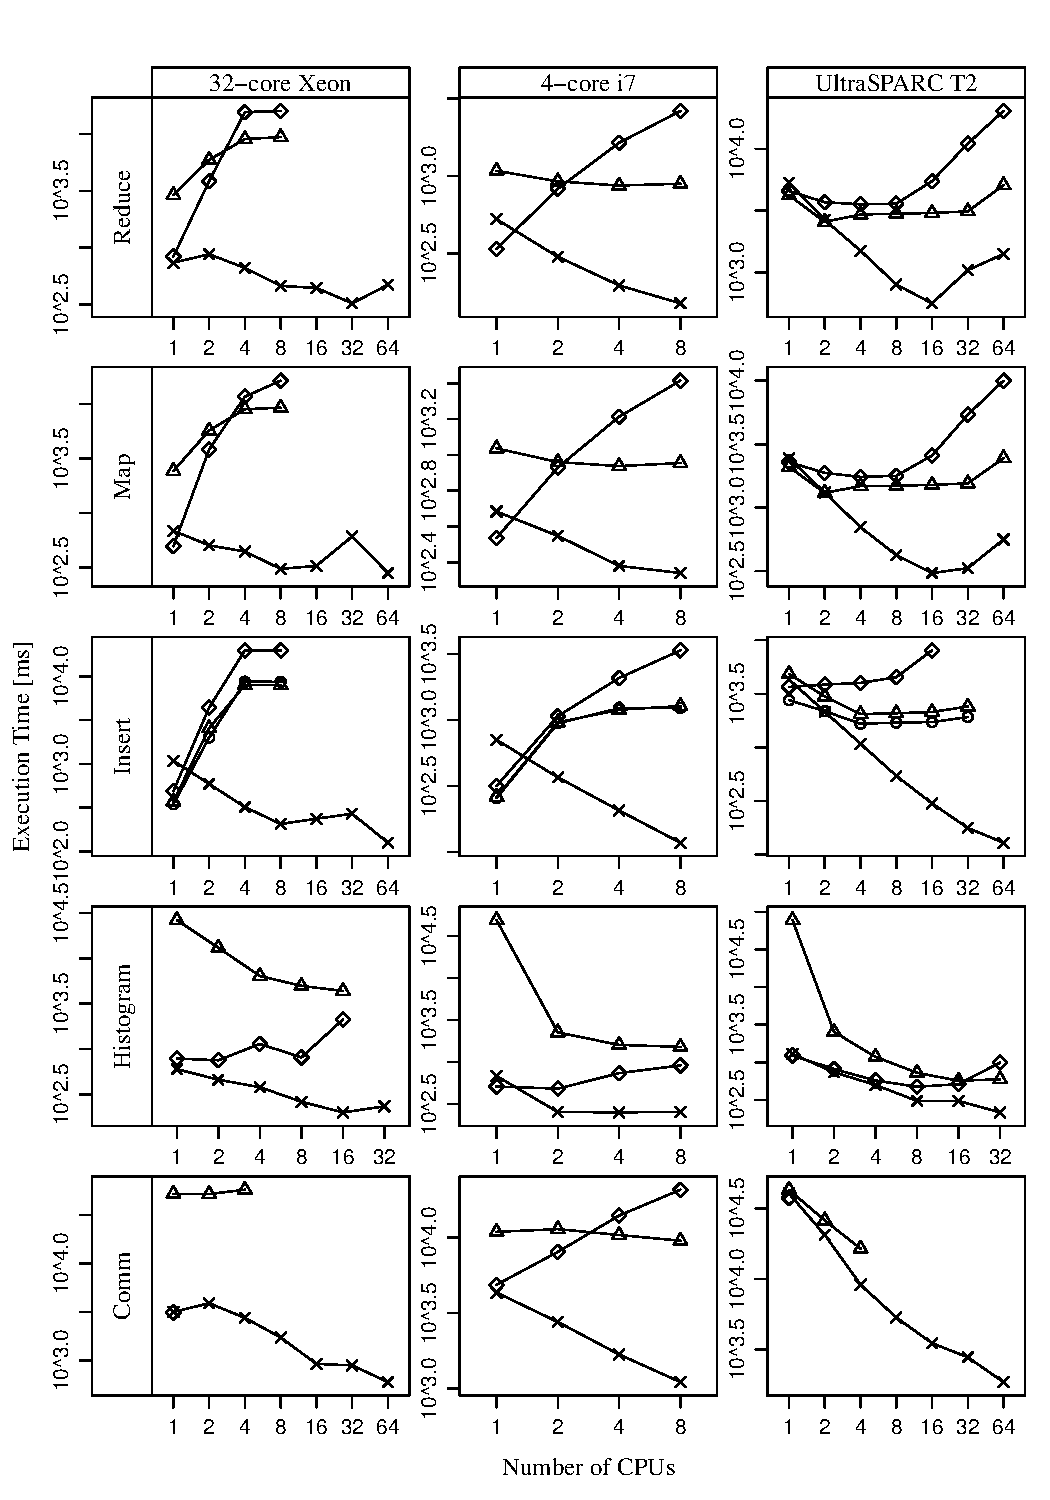
\includegraphics[width=\textwidth]{../benchmarks/graphs/cpu-scaling}
\caption{CPU scaling properties of benchmarks}
\end{figure}

\begin{figure}
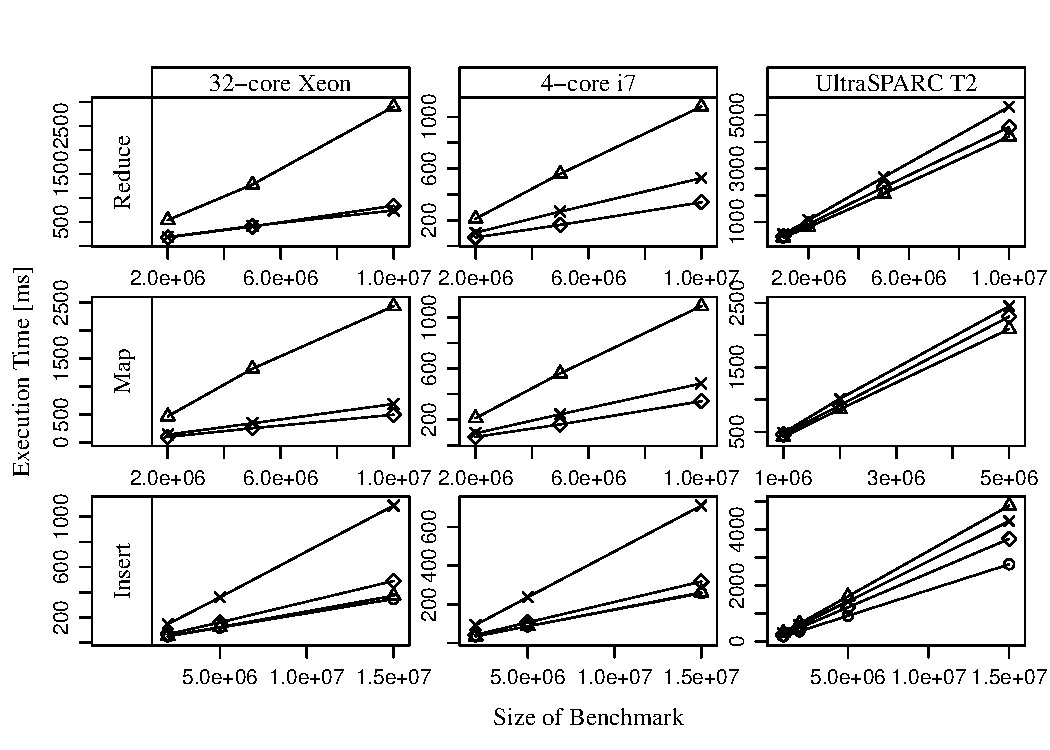
\includegraphics[width=\textwidth]{../benchmarks/graphs/size-scaling-par1}
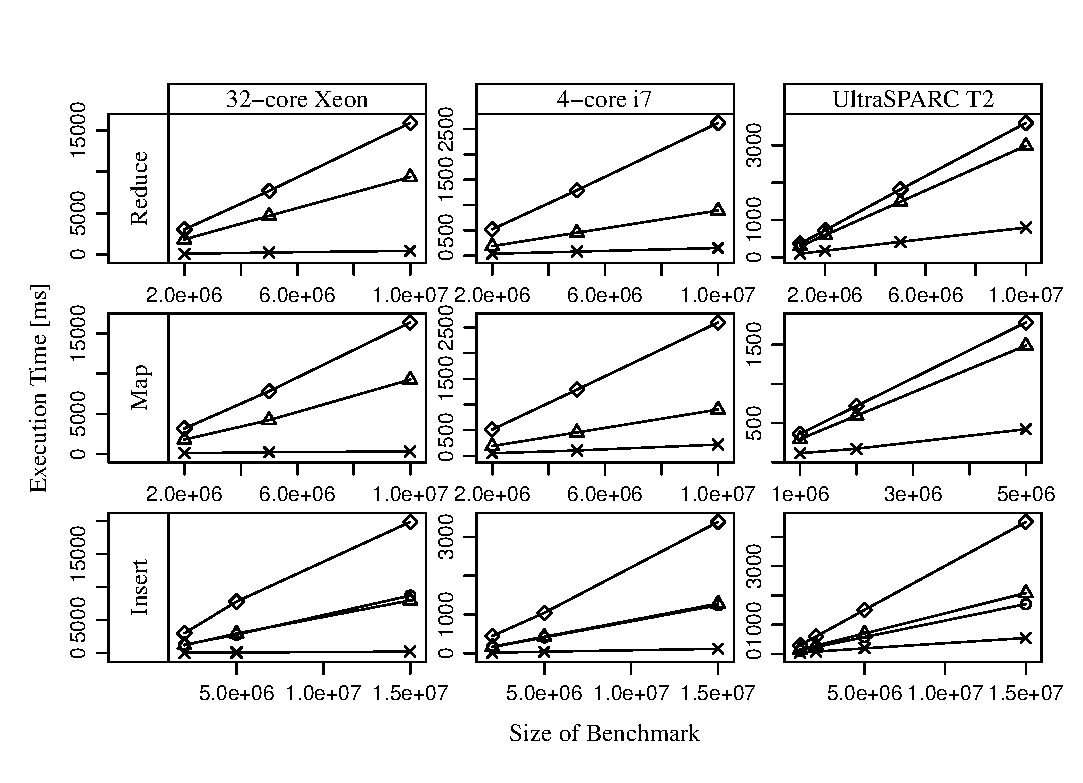
\includegraphics[width=\textwidth]{../benchmarks/graphs/size-scaling-par8}
\caption{Size scaling properties of benchmarks ($P = 1, 8$)}
\end{figure}

\begin{figure}
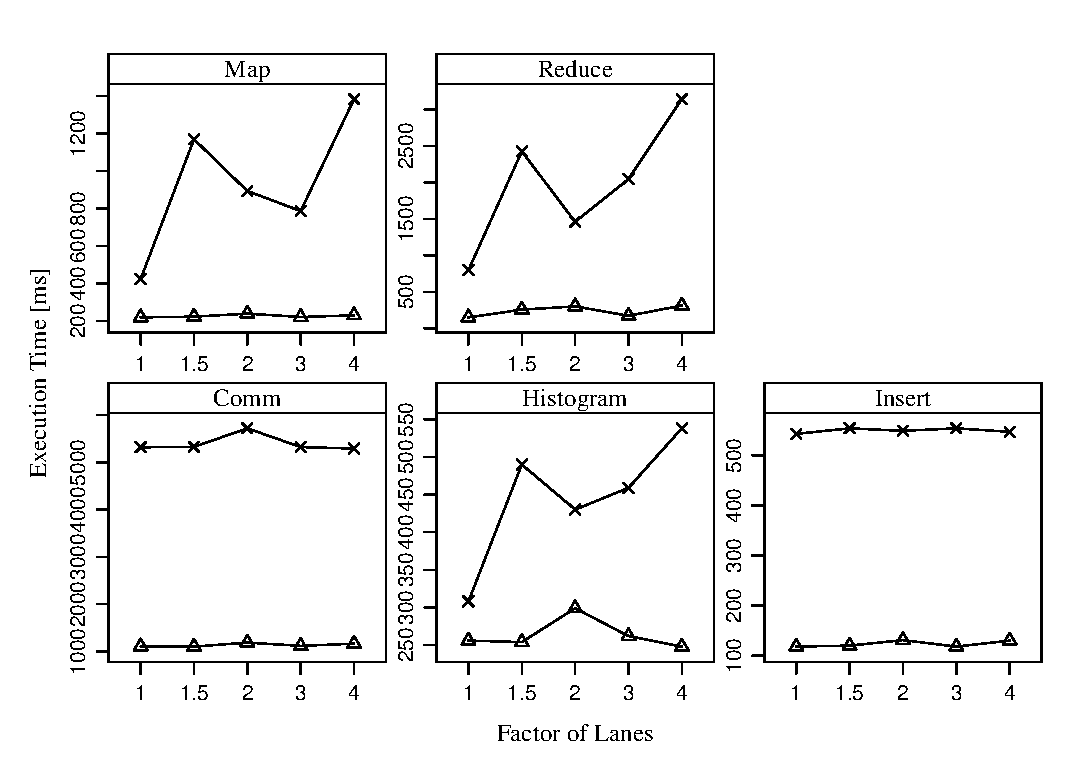
\includegraphics[width=\textwidth]{../benchmarks/graphs/lanef-scaling}
\caption{Lane-Factor scaling properties of Multi-Lane FlowPool}
\end{figure}

\section{Related Work}

An introduction to linearizability, lock-freedom and basic
concurrent programming techniques is given by Herlihy and Shavit
\cite{Herlihy08}.
A detailed overview of concurrent data structures is given
by Moir and Shavit \cite{Moir05}.
To date, concurrent data structures remain an active area of
research -- it is out of scope to list them all, so we restrict
ourselves to those relevant to this work.

Concurrently accessible queues have been present for a while --
an implementation is described by \cite{Mellor87}.
Non-blocking concurrent linked queues are described by Michael and
Scott \cite{Michael96}. This CAS-based linked-list
queue implementation is cited and used widely today, a variant of
which is present in the Java standard library.
More recently, Scherer, Lea and Scott \cite{SchererLS09} describe a
synchronous queues which internally hold both data and requests.
Both approaches above entail blocking (or spinning) at least on the
consumer's part when the queue is empty.

While the abstractions above fit well in the concurrent imperative
model, they have the disadvantage that the programs written using them
are inherently nondeterministic.
Book by Roy and Haridi \cite{RoyH2004} describes the Oz programming language 
a subset of which yields programs deterministic by construction.
The Oz dataflow streams are built on top of
single-assignment variables and are deterministically ordered.
They allow multiple consumers, but only one producer
at a time.
Oz has its own runtime which implements blocking using
continuations.
Blocking is less efficient on the JVM, CLR and many native
environments.

The concept of single-assignment variables is also embodied in
futures proposed by Baker and Hewitt \cite{Hewitt77}, and promises
first mentioned by Friedman and Wise \cite{Wise76}.
Futures were first implemented in MultiLISP \cite{Halstead85},
and have been employed in many languages and frameworks since.
Scala futures \cite{TODO} and Finagle futures \cite{TODO} are
of interest, because they define monadic operators and a
number of high-level combinators which produce new futures.
This provides an API which avoids blocking.
Futures have been generalized to data-driven futures,
which can provide additional information to the scheduler
\cite{Tasirlar11}.
Many frameworks have constructs which start an asynchronous
computation and yield a future holding its result.
For example, Habanero Java \cite{Shirako11} offers an \verb=async=
construct and Scala futures offer a \verb=future= construct.

A number of other models and frameworks recognized the need to embed
the concept of futures into other data-structures.
Single-assignment variables have been generalized to I-Structures
proposed by Arvind \cite{Arvind89} which are essentially
single-assignment arrays.
The CnC model \cite{Burke11} \cite{CnC10} is a parallel programming model
influenced by dynamic dataflow, stream-processing and tuple spaces.
In CnC the user provides high-level operations along with the ordering
constraints that form a computation dependency graph.
FlumeJava \cite{Chambers10} is a distributed programming model which
relies heavily on the concept of collections containing a set of
futures.
An issue that often arises with dataflow programming models are
unbalanced loads.
This is often solved through the use of bounded buffers which prevent
the producer from overflowing the consumer.
Analytical approaches to modeling pipelined applications have also
been addressed \cite{Cascaval09}.

Opposed to the correct-by-construction determinism described thus far,
a type-systematic approach can also ensure that concurrent executions
have deterministic results.
Recently, work on Deterministic Parallel Java showed that a
region-based type system can ensure determinism \cite{Bocchino09}.
X10's constrained-based dependent types can similarly ensure
determinism and deadlock-freedom \cite{Saraswat07}.


\section{Conclusion}

We have shown that deterministic higher-level operations can be build
on top of \verb=<<= and \verb=foreach=, which corresponds to
sequential collections.
The prerequisite is that \verb=<<= can be invoked concurrently and
that \verb=foreach= executes asynchronously.

We emphasize a property of FlowPools which goes beyond
a dataflow model such as Oz (or some other future/promise based
model) in which more complex data structures such as streams are built
on top of single-assignment variables.
With single-assignment pools multiple threads can add elements without
agreeing on where the added element should structurally be, as is the
case with dataflow streams.
A consequence of this is a more flexible programming model.

In conclusion, we postulate the existence of a range of other
concurrent collection types with deterministic semantics fitting the
presented correct-by-construction single-assignment model, such as
bounded buffers, dataflow streams and maps, all of which have
higher-level operations expressed in terms of the same basic
primitives.
On the implementation level, we anticipate the need of embedding the
callbacks within the data-structure itself, as is the case with
callback-based futures and FlowPools -- this offers a particular
benefit on platforms which do not by default support efficient
continuations.



\bibliographystyle{abbrv}
\bibliography{bib}

\appendix
\section{Proof of Correctness}


\setcounter{lemma}{0}
\setcounter{theorem}{0}
\setcounter{corollary}{0}
\setcounter{definition}{0}




\begin{definition}[Data types]
A \textbf{Block} $b$ is an object which
contains an array $b.array$, which itself can contain elements, $e \in Elem$,
where \textbf{Elem} represents the type of $e$ and can be any countable set. A
given block $b$ additionally contains an index $b.index$ which represents an
index location in $b.array$, a unique index identifying the array
$b.blockIndex$, and $b.next$, a reference to a successor block $c$ where
$c.blockIndex = b.blockIndex + 1$. A \textbf{Terminal} $term$ is a sentinel
object, which contains an integer $term.sealed \in \{-1\} \cup \mathbb{N}_0$, and
$term.callbacks$, a set of functions $f \in Elem \Rightarrow Unit$.

We define the following functions:

\begin{equation*}
following(b: Block) = 
\begin{cases}
\emptyset & \text{if b.next = null,}
\\
b.next \cup following(b.next) & \text{otherwise}
\end{cases}
\end{equation*}

\begin{equation*}
reachable(b: Block) = \{ b \} \cup following(b)
\end{equation*}

\begin{equation*}
last(b: Block) = b' : b' \in reachable(b) \wedge b'.next = null
\end{equation*}

\begin{equation*}
size(b: Block) = | \{ x : x \in b.array \wedge x \in Elem \} |
\end{equation*}

Based on them we define the following relation:

\begin{equation*}
reachable(b, c) \Leftrightarrow c \in reachable(b)
\end{equation*}
\end{definition}


\begin{definition}[FlowPool]
A \textbf{FlowPool} $pool$ is an object that
has a reference $pool.start$, to the first block $b_0$ (with $b_0.blockIndex=0$), 
as well as a reference $pool.current$.
We sometimes refer to these just as $start$ and $current$, respectively.

A \textbf{scheduled callback invocation} is a pair $(f, e)$ of a function
$f \in Elem => Unit$ and an element $e \in Elem$.
The programming construct that adds such a pair to the set of
$futures$ is \verb=future { f(e) }=.

The \textbf{FlowPool state} is defined as a pair of the directed graph of
objects transitively reachable from the reference $start$ and the set
of scheduled callback invocations called $futures$.

A \textbf{state changing} or \textbf{destructive} instruction is any
atomic write or CAS instruction that changes the FlowPool state.

We say that the FlowPool \textbf{has an element} $e$ at some time
$t_0$ if and only if the relation $hasElem(start, e)$ holds.

\begin{equation*}
hasElem(start, e) \Leftrightarrow \exists b \in reachable(start), e
\in b.array
\end{equation*}

We say that the FlowPool \textbf{has a callback} $f$ at some time
$t_0$ if and only if the relation $hasCallback(start, f)$ holds.

\begin{equation*}
hasCallback(start, f) \Leftrightarrow \forall b = last(start), b.array
= x^P \cdot t \cdot y^N, x \in Elem, t = Terminal(seal, callbacks), f
\in callbacks
\end{equation*}

We say that a callback $f$ in a FlowPool \textbf{will be called} for
the element $e$ at some time $t_0$ if and only if the relation
$willBeCalled(start, e, f)$ holds.

\begin{equation*}
willBeCalled(start, e, f) \Leftrightarrow \exists t_1, \forall t >
t_1, (f, e) \in futures
\end{equation*}

We say that the FlowPool is \textbf{sealed} at the size $s$ at some
$t_0$ if and only if the relation $sealedAt(start, s)$ holds.

\begin{equation*}
sealedAt(start, s) \Leftrightarrow s \neq -1 \wedge \forall b = last(start), b.array
= x^P \cdot t \cdot y^N, x \in Elem, t = Terminal(s, callbacks)
\end{equation*}

\textbf{FlowPool operations} are \verb=append=, \verb=foreach= and
\verb=seal=, and are defined by pseudocodes in figures ...
\end{definition}


\begin{definition}[Invariants]
We define the following invariants for the \textbf{FlowPool}:
\begin{description}
\item[INV1] $start = b: Block, b \neq null, current \in reachable(start)$
\item[INV2] $\forall b \in reachable(start), b \not \in following(b)$
\item[INV3] $\forall b \in reachable(start), b \neq last(start) \Rightarrow size(b) = LASTELEMPOS \wedge b.array(BLOCKSIZE - 1) \in Terminal$
\item[INV4]
$\forall b = last(start), b.array = p \cdot c \cdot n$, where:

$p = X^P, c = c_1 \cdot c_2, n = null^N$

$x \in Elem, c_1 \in Terminal, c_2 \in \{null\} \cup Terminal$

$P + N + 2 = BLOCKSIZE$
\item[INV5] $\forall b \in reachable(start), b.index > 0 \Rightarrow b.array(b.index - 1) \in Elem$
\end{description}
\end{definition}


\begin{definition}[Validity]
A FlowPool state $\mathbb{S}$ is \textbf{valid} if and only if the invariants [INV1-5] hold for that state.
\end{definition}


\begin{definition}[Abstract pool]
An \textbf{abstract pool} $\mathbb{P}$ is a function from time $t$ to a tuple $(elems, callbacks, seal)$ such that:
\begin{description}
\item $seal \in \{ -1 \} \cup \mathbb{N}_0$
\item $callbacks \subset \{ (f: Elem => Unit, called) \}$
\item $called \subseteq elems \subseteq Elem$
\end{description}
We say that an abstract pool $\mathbb{P}$ \textbf{is in state}
$\mathbb{A} = (elems, callbacks, seal)$ at time $t$ if and only if $\mathbb{P}(t) = (elems, callbacks, seal)$.
\end{definition}


\begin{definition}[Abstract pool operations]
We say that an \textbf{abstract pool operation} $op$ applied to an
abstract pool $\mathbb{P}$ in abstract state $\mathbb{A}_0 = (elems_0, callbacks_0, seal_0)$ 
at some time $t$ \textbf{changes} the abstract state of the abstract pool to $\mathbb{A} = (elems, callbacks, seal)$ 
if $\exists t_0, \forall \tau, t_0 < \tau < t, \mathbb{P}(\tau) = \mathbb{A}_0$
and $\mathbb{P}(t) = \mathbb{A}$.
We denote this as $\mathbb{A} = op(\mathbb{A}_0)$.

Abstract pool operation $foreach(f)$ changes the abstract state at $t_0$ from $(elems, callbacks, seal)$ 
to $(elems, (f, \emptyset) \cup callbacks, seal)$. Furthermore:

$\exists t_1 \geq t_0, \forall t_2 > t_1, \mathbb{P}(t_2) = (elems_2,
callbacks_2, seal_2) \wedge \forall (f, called_2) \in callbacks_2,
elems \subseteq called_2 \subseteq elems_2$

Abstract pool operation $append(e)$ changes the abstract state at $t_0$ from
$(elems, callbacks, seal)$ to $(\{e\} \cup elems, callbacks, seal)$. Furthermore:

$\exists t_1 \geq t_0, \forall t_2 > t_1, \mathbb{P}(t_2) = (elems_2,
callbacks_2, seal_2) \wedge \forall (f, called_2) \in callbacks_2,
(f, called) \in callbacks \Rightarrow elem \in called_2$

Abstract pool operation $seal(s)$ changes the abstract state at $t_0$ from
$(elems, callbacks, seal)$ to $(elems, callbacks, s)$, assuming
that $seal \in \{-1\} \cup \{s\}$ and $s \in \mathbb{N}_0$, and
$|elems| \leq s$.
\end{definition}


\begin{definition}[Consistency]
A FlowPool state $\mathbb{S}$ is \textbf{consistent} with an abstract pool 
$\mathbb{P} = (elems, callbacks, seal)$ at $t_0$ if and only if $\mathbb{S}$ 
is a valid state and:
\begin{description}
\item $\forall e \in Elem, hasElem(start, e) \Leftrightarrow e \in elems$
\item $\forall f \in Elem => Unit, hasCallback(start, f) \Leftrightarrow f \in callbacks$
\item $\forall f \in Elem => Unit, \forall e \in Elem, willBeCalled(start, e, f) \Leftrightarrow \exists t_1 \geq t_0, \mathbb{P}(t_1) = (elems_1, (f, called_1) \cup callbacks_1, seal_1), elems \subseteq called_1$
\item $\forall s \in \mathbb{N}_0, sealedAt(start, s) \Leftrightarrow s = seal$
\end{description}

A FlowPool operation $op$ is \textbf{consistent} with the corresponding 
abstract state operation $op'$ if and only if $\mathbb{S'}=op(\mathbb{S})$ is consistent 
with an abstract state $\mathbb{A'}=op'(\mathbb{A})$.

A \textbf{consistency change} 
is a change from state $\mathbb{S}$ to state $\mathbb{S'}$ such that $\mathbb{S}$ 
is consistent with an abstract state $\mathbb{A}$ and $\mathbb{S'}$ is consistent 
with an abstract set $\mathbb{A'}$, where $\mathbb{A} \neq \mathbb{A'}$.

%A FlowPool operation $op$ completing at some time $t_0$ is \textbf{consistent} with an abstract pool operation $op'$ if 
%and only if $op$ changes the state of the FlowPool from $\mathbb{S}_1$ to $\mathbb{S}_2$, where $\mathbb{S}_1$ 
%and $\mathbb{S}_2$ are consistent with the abstract pool states $\mathbb{A}_1$ and $\mathbb{A}_2$, respectively, 
%and $op'$ changes the state of the abstract pool from $\mathbb{A}_1$ to $\mathbb{A}_2$.
\end{definition}


\begin{proposition}
Every valid state is consistent with some abstract pool.
\end{proposition}


\begin{theorem}[Safety]
FlowPool operation \verb=create= creates a new FlowPool consistent with the abstract pool 
$\mathbb{P} = (\emptyset, \emptyset, -1)$. FlowPool operations \verb=foreach=, \verb=append= 
and \verb=seal= are consistent with the abstract pool semantics.
\end{theorem}


\begin{lemma}[End of life]\label{lemma-end-of-life}
For all blocks $b \in reachable(start)$, if value $v \in Elem$ is
written to $b.array$ at some position $idx$ at some time $t_0$, then
$\forall t > t_0, b.array(idx) = v$.
\end{lemma}

\begin{proof}
The CAS in line \ref{cas_append} is the only CAS which writes an
element.
No other CAS has a value of type $Elem$ as the expected value.
This means that once the CAS in line \ref{cas_append} writes a value
of type $Elem$, no other write can change it.
\end{proof}


\begin{corollary}\label{cor-end-of-life}
The end of life lemma implies that if all the values in $b.array$ are
of type $Elem$ at $t_0$, then $\forall t > t_0$ there is no write to $b.array$.
\end{corollary}


\begin{lemma}[Valid hint]\label{lemma-valid-hint}
For all blocks $b \in reachable(start)$, if $b.index > 0$ at some time $t_0$, then
$b.array(b.index - 1) \in Elem$ at time $t_0$.
\end{lemma}

\begin{proof}
Observe every write to $b.index$ -- they are all unconditional.
However, at every such write occurring at some time $t_1$ that writes
some value $idx$ we know that some previous value at $b.array$ entry $idx - 1$
at some time $t_0 < t_1$ was of type $Elem$.
Hence, from lemma \ref{lemma-end-of-life} it follows that
$\forall t \geq t_1, b.array(idx - 1) \in Elem$.
\end{proof}


\begin{corollary}[Compactness]\label{cor-compactness}
For all blocks $b \in reachable(start)$, if for some $idx$
$b.array(idx) \in Elem$ at time $t_0$ then $b.array(idx - 1) \in Elem$
at time $t_0$. This follows
directly from the lemmas \ref{lemma-end-of-life} and
\ref{lemma-valid-hint}, and the fact that the CAS in line
\ref{cas_append} only writes to array entries $idx$ for which it
previously read the value from $b.index$.
\end{corollary}


\begin{definition}[Transition]
If for a function $f(t)$ there exist times $t_0$ and $t_1$ such that
$\forall t, t_0 < t < t_1, f(t) = v_0$ and $f(t_1) = v_1$, then we say
that the function $f$ goes through a \textbf{transition} at $t_1$. We denote this as:

$f: v_0 \stackrel{t_1}{\rightarrow} v_1$

Or, if we don't care about the exact time $t_1$, simply as:

$f: v_0 \rightarrow v_1$
\end{definition}


\begin{definition}[Monotonicity]
A function of time $f(t)$ is said to be \textbf{monotonic}, if every value in its string of transitions occurs only once.
\end{definition}


\begin{lemma}[Freshness]\label{lemma-freshness}
For all blocks $b \in reachable(start)$, and for all $x \in b.array$,
function $x$ is monotonic.
\end{lemma}

\begin{proof}
CAS instruction in line \ref{cas_append} writes a value of type
$Elem$. No CAS instruction has a value of type $Elem$ as the expected value.

Trivial analysis of CAS instructions in lines \ref{cas_seal} and
\ref{cas_callback}, shows that their expected values are of type
$Terminal$. Their new values are always freshly allocated.

The more difficult part is to show that CAS instruction in line
\ref{cas_propagate} respects the statement of the lemma.

Since the CAS instructions in lines \ref{cas_seal} and
\ref{cas_callback} are preceeded by a read of $idx = b.index$,
from lemma \ref{lemma-valid-hint} it follows that $b.array(idx - 1)$ 
contains a value of type $Elem$.
These are also the only CAS instructions which replace a $Terminal$
value with another $Terminal$ value. The new value is always unique, as
shown above.

So the only potential CAS to write a non-fresh value to $idx + 1$ is the CAS
in line \ref{cas_propagate}.

A successful CAS in line \ref{cas_propagate} overwrites a value $cb_0$ at $idx + 1$
read in line \ref{read_next} at $t_0$ with a new value $cb_2$ at time $t_2$. Value $cb_2$ was
read in line \ref{read_current} at $t_1$ from the entry $idx$. The
string of transitions of values at $idx$ is composed of unique values
at least since $t_1$ (by lemma \ref{lemma-end-of-life}), since there is
a value of type $Elem$ at the index $idx - 1$.

The conclusion above ensures that the values read in line \ref{read_current}
to be subsequently used as new values for the CAS in line \ref{cas_propagate}
form a monotonic function $f(t) = b.array(idx) \text{ at } t$.

Now assume that a thread T1 successfully overwrites $cb_0$
via CAS in line \ref{cas_propagate} at $idx + 1$ at time $t_2$ 
to a value $cb_2$ read from $idx$ at $t_1$, and that another thread T2 
is the \textbf{first} thread (since the FlowPool was created) to subsequently successfully
complete the CAS in line \ref{cas_propagate} at $idx + 1$ at time
$t_{prev2} > t_2$ with some value $cb_{prev2}$ which was at $idx + 1$ at some time
$t < t_0$.

That would mean that $b.array(idx + 1)$ does not change during $\langle t_0, t_2 \rangle$,
since T2 was the first thread the write a non-fresh value to $idx + 1$, and any
other write would cause the CAS in line \ref{cas_propagate} by T1 to fail.
%That means that $t_0 > t_{prev0}$, otherwise the CAS in line \ref{cas_propagate}
%by T2 would have failed.

Also, that would mean that the thread T2 read the value
$cb_{prev2}$ in line \ref{read_current} at some time $t_{prev1} < t_1$
and successfully completed the CAS at time $t_{prev2} > t_2$. If the
CAS was successful, then the read in line \ref{read_next} by T2
occured at $t_{prev0} < t_{prev1} < t_1$. Since we assumed that T2 is the
first thread to write a value $cb_{prev2}$ to $idx + 1$ at time $t_{prev2}$
which was previously in $idx + 1$ at some time $t < t_0$, then the CAS
in line \ref{cas_propagate} at time $t_{prev2}$ could not have succeeded,
since its expected value is $cb_{prev0}$ read at some time $t_{prev0}$, and
we know that the value at $idx + 1$ was changed at least once in $\langle t_{prev0}, t_{prev2} \rangle$
because of the write of a fresh value by thread T1 at $t_2 \in \langle t_{prev0}, t_{prev2} \rangle$.
This value is known to be fresh because $b.array(idx)$ is a monotonic
function at least since $t_{prev1}$, and the read of the new value
written by T1 occurred at $t_1 > t_{prev1}$.
We also know that there is no other thread T3 to write the value
 $cb_{prev0}$ during $\langle t_{prev0}, t_{prev2} \rangle$
back to $idx + 1$, since we assumed that T2 is the first to write
a non-fresh value at that position.

Hence, a contradiction shows that there is no thread T2 which is the \textbf{first}
to write a non-fresh value via CAS in line \ref{cas_propagate} at $idx + 1$
for any $idx$, so there is no thread that writes a non-fresh value at all.
\end{proof}


\begin{lemma}[Lifecycle]\label{lemma-lifecycle}
For all blocks $b \in reachable(start)$, and for all $x \in b.array$, function $x$ goes through and only through the prefix of the following transitions:

$null \rightarrow cb_1 \rightarrow \dots \rightarrow cb_n \rightarrow elem$, where:

$cb_i \in Terminal, i \neq j \Rightarrow cb_i \neq cb_j, elem \in Elem$
\end{lemma}

\begin{proof}
First of all, it is obvious from the code that each block that becomes
an element of $reachable(start)$ at some time $t_0$ has the value of
all $x \in b.array$ set to $null$.

Next, we inspect all the CAS instructions that operate on entries of
$b.array$.

The CAS in line \ref{cas_append} has a value $curo \in Terminal$ as
an expected value and writes an $elem \in Elem$.
This means that the only transition that this CAS
can cause is of type $cb_i \in Terminal \rightarrow elem \in Elem$.

We will now prove that the CAS in line \ref{cas_propagate} at time $t_2$ is successful if and
only if the entry at $idx + 1$ is $null$ or $nexto \in
Terminal$.
We know that the entry at $idx + 1$ does not change $\forall t, t_0 < t < t_2$,
where $t_0$ is the read in line \ref{read_next},
because of lemma \ref{lemma-freshness} and the fact that CAS in line \ref{cas_propagate} is assumed to be successful.
We know that during the read in line \ref{read_current} at time $t_1$,
such that $t_0 < t_1 < t_2$, the entry at $idx$ was $curo \in
Terminal$, by trivial analysis of the \verb=check= procedure.
It follows from corollary \ref{cor-compactness} that the array entry $idx
+ 1$ is not of type $Elem$ at time $t_1$, otherwise array entry $idx$
would have to be of type $Elem$.
Finally, we know that the entry at $idx + 1$ has the same value during
the interval $\langle t_1, t_2 \rangle$, so its value is not $Elem$ at $t_2$.

The above reasoning shows that the CAS in line \ref{cas_propagate}
always overwrites a one value of type $Terminal$ (or $null$) with
another value of type $Terminal$.
We have shown in lemma \ref{lemma-freshness} that it never
overwrites the value $cb_0$ with a value $cb_2$ that was at
$b.array(idx)$ at an earlier time.

Finally, note that the statement for CAS instructions in lines \ref{cas_seal} and
\ref{cas_callback} also follows directly from the proof for lemma \ref{lemma-freshness}.
\end{proof}


\begin{lemma}[Subsequence]\label{lemma-subsequence}
Assume that for some block $b \in reachable(start)$ the transitions of
$b.array(idx)$ are:

\begin{equation*}
b.array(idx): null \rightarrow cb_1 \rightarrow \cdots \rightarrow
cb_n \stackrel{t_0}{\rightarrow} elem: Elem
\end{equation*}

Assume that the transitions of $b.array(idx + 1)$ up to time $t_0$ are:

\begin{equation*}
b.array(idx + 1): null \rightarrow cb_1' \rightarrow \cdots
\rightarrow cb_m'
\end{equation*}

The string of transitions $null \rightarrow cb_1' \rightarrow \cdots
\rightarrow cb_m'$ is a subsequence of $null \rightarrow cb_1
\rightarrow \cdots \rightarrow cb_n$.
\end{lemma}

\begin{proof}
Note that all the values written to $idx + 1$ before $t_0$ by CAS in line \ref{cas_propagate} were
previously read from $idx$ in line \ref{read_current}.
This means that the set of values occurring in $b.array(idx + 1)$
before $t_0$ is a subset of the set of values in $b.array(idx)$.
We have to prove that it is actually a subsequence.

Assume that there exist two values $cb_1$ and $cb_2$ read by threads T1 and T2
in line \ref{read_current} at times $t_1$ and $t_2 > t_1$, respectively.
Assume that these values are written to $idx + 1$ by threads T1 and T2
in line \ref{cas_propagate} in the opposite order, that is at times
$t_{cas1}$ and $t_{cas2} < t_{cas1}$, respectively.
That would mean that the CAS by thread T1 would have to fail, since its expected
value $cb_0$ has changed between the time it was read in line \ref{read_next} and
the $t_{cas1}$ at least once to a different value, and it could not have been
changed back to $cb_0$ as we know from the lemma
\ref{lemma-freshness}.

Notice that we have actually prooved a stronger result above.
We have also shown that the string of values
written at $idx + 1$ by CAS in line \ref{cas_propagate} successfully is a subsequence
of \textbf{all} the transitions of values at $idx$ (not just until $t_0$).
\end{proof}


\begin{lemma}[Valid writes]\label{lemma-valid}
Given a FlowPool in a valid state, all writes in all operations produce a FlowPool in a valid state.
\end{lemma}

\begin{proof}
A new FlowPool is trivially in a valid state.

Otherwise, assume that the FlowPool is in a valid state
$\mathbb{S}$.
In the rest of the proof, whenever some invariant is trivially
unaffected by a write, we omit mentioning it.
We start by noting that we already prooved the claim
for atomic writes in lines \ref{write_append}, \ref{write_advance} and
\ref{write_seal} (which only affect [INV5]) in lemma
\ref{lemma-valid-hint}.
We proceed by analyzing each atomic CAS instruction.

CAS in line \ref{cas_expand} at time $t_1$ maintains the invariant
[INV1].
This is because its expected value is always
$null$, which ensures that the lifecycle of $b.next$ is $null
\rightarrow b': Block$, meaning that the function $reachable(start)$
returns a monotonically growing set.
So if $current \in reachable(start)$ at $t_0$, then this also holds at
$t_1 > t_0$.
It also maintains [INV2] because the new value $nb$ is always fresh,
so $\forall b, b \not \in following(b)$.
Finally, it maintains [INV3] because it is preceeded with a bounds
check and we know from corollary \ref{cor-compactness} and the
lemma \ref{lemma-end-of-life} that all the values in $b.array(idx),
idx < LASTELEMPOS$ must be of type $Elem$.

CAS in line \ref{cas_block} at time $t_1$ maintains the
invariant [INV1], since the new value for the $current \neq null$ was read from
$b.next$ at $t_0 < t_1$ when the invariant was assumed to hold, and
it is still there a $t_1$, as shown before.

For CAS instructions in lines \ref{cas_append}, \ref{cas_callback} and
\ref{cas_seal} that write to index $idx$ we know from lemma
\ref{lemma-valid-hint} that the value at $idx - 1$ is of type $Elem$.
This immediately shows that CAS instructions in lines
\ref{cas_callback} and \ref{cas_seal} maintain [INV3] and [INV4].

For CAS in line \ref{cas_append} we additionally know that it must
have been preceeded by a successful CAS in line \ref{cas_propagate}
which previously wrote a $Terminal$ value to $idx + 1$. From lemma
\ref{lemma-lifecycle} we know that $idx + 1$ is still $Terminal$ when
the CAS in line \ref{cas_append} occurs, hence [INV4] is kept.

Finally, CAS in line \ref{cas_propagate} succeeds only if the value at
$idx + 1$ is of type $Terminal$, as shown before in lemma
\ref{lemma-lifecycle}.
By the same lemma, the value at $idx$ is either
$Terminal$ or $Elem$ at that point, since $idx - 1$ is known to be
$Elem$ by lemma \ref{lemma-valid-hint}.
This means that [INV4] is kept.
\end{proof}


\begin{lemma}[Housekeeping]\label{lemma-housekeeping}
Given a FlowPool in state $\mathbb{S}$ consistent with some abstract
pool state $\mathbb{A}$, CAS instructions in lines \ref{cas_propagate}, \ref{cas_expand} and
\ref{cas_block} do not change the abstract pool state $\mathbb{A}$.
\end{lemma}

\begin{proof}
Since none of the relations $hasElem$, $hasCallback$, $willBeCalled$ and $sealedAt$
are defined by the value of $current$ CAS in line \ref{cas_block}
does not change them, hence it does not change the abstract pool
state.

No CAS changes the set of scheduled futures, nor is
succeeded by a \verb=future= construct so it does not affect
the $willBeCalled$ relation.

It is easy to see that the CAS in line \ref{cas_expand} does not remove any elements, nor make
any additional elements reachable, since the new block $nb$ which
becomes reachable does not contain any elements at that time.
Hence the $hasElem$ relation is not affected.
It does change the value $last(start)$ to $nb$, but since $nb.array =
t \cdot null^{BLOCKSIZE - 1}$, where $t \in Terminal$ was previously
the last non-null element in $b.array$, it does changes neither the
$sealedAt$ nor the $hasCallback$ relation.

The CAS in line \ref{cas_propagate} does not make some new element reachable,
hence the $hasElem$ relation is preserved.

Note now that this CAS does not change the relations $hasCallback$
and $sealedAt$ as long as there is a value of type $Terminal$ at the
preceeding entry $idx$.
We claim that if the CAS succeeds at $t_2$, then 
either the value at $idx$ is of type $Terminal$ (trivially) or the CAS
did not change the value at $idx + 1$.
In other words, if the value at $idx$ at time $t_2$ is of type $Elem$,
then the write by CAS in line \ref{cas_propagate} does not change
the value at $idx + 1$ at $t_2$.
This was, in fact, already shown in the proof of lemma \ref{lemma-subsequence}.

The argument above proves directly that relations $hasCallback$
and $sealedAt$ are not changed by the CAS in line \ref{cas_propagate}.
\end{proof}


\begin{lemma}[Append correctness]\label{lemma-append}
Given a FlowPool in state $\mathbb{S}$ consistent with some abstract pool state $\mathbb{A}$, 
a successful CAS in line \ref{cas_append} at some time $t_0$ changes the state of the FlowPool 
to $\mathbb{S}_0$ consistent with an abstract pool state $\mathbb{A}_0$, such that:

$\mathbb{A} = (elems, callbacks, seal)$

$\mathbb{A}_0 = (\{elem\} \cup elems, callbacks, seal)$

Furthermore, given a fair scheduler, there exists a time $t_1 > t_0$ at which the FlowPool 
is consistent with an abstract pool in state $\mathbb{A}_1$, such that:

$\mathbb{A}_1 = (elems_1, callbacks_1, seal_1)$, where:

$\forall (f, called_1) \in callbacks_1, (f, called) \in callbacks \Rightarrow elem \in called_1$
\end{lemma}

\begin{proof}
Assume that the CAS in line \ref{cas_append} succeeds at some time
$t_3$, the CAS in line \ref{cas_propagate} succeeds at some time $t_2 <
t_3$, the read in line \ref{read_current} occurs at some time $t_1 <
t_2$ and the read in line \ref{read_current} occurs at some time $t_0
< t_1$.

It is easy to see from the invariants, $check$ procedure and the
corollary \ref{cor-end-of-life} that the CAS in line \ref{cas_append} can only
occur if $b = last(start)$.

We claim that for the block $b \in reachable(start)$ such that $b = last(b)$ the
following holds at $t_2$:

$b.array = elem^N \cdot cb_1 \cdot cb_2 \cdot null^{BLOCKSIZE - N - 2}$

where $cb_1 = cb_2$, since there was no write to $idx$ after $cb_1$, otherwise the
CAS in line \ref{cas_append} at $t_3$ would not have been successful
(by lemma \ref{lemma-freshness}).

Furthermore, $cb_1 = cb_2$ at $t_3$, as shown in the lemma
\ref{lemma-subsequence}. Due to the same lemma, the entries of
$b.array$ stay the same until $t_3$, otherwise the CAS in line
\ref{cas_append} would not have been successful.
After the successful CAS at $t_3$, we have:

$b.array = elem^N \cdot e \cdot cb_1 \cdot null^{BLOCKSIZE - N - 2}$

where $e: Elem$ is the newly appended element-- at $t_3$ the relation
$hasElem(start, e)$ holds, and $sealedAt(start, s)$ and $hasCallback(start,
f)$ did not change between $t_2$ and $t_3$.

It remains to be shown that $willBeCalled(start, e, f)$ holds at $t_3$.
Given a fair scheduler, within a finite number of steps the
future store will contain a request for an asynchronous computation
that invokes $f$ on $e$. The fair scheduler ensures that the future is
scheduled within a finite number of steps.
\end{proof}


\begin{lemma}[Foreach correctness]\label{lemma-foreach}
Given a FlowPool in state $\mathbb{S}$ consistent with some abstract pool state $\mathbb{A}$, 
a successful CAS in line \ref{cas_callback} at some time $t_0$ changes the state of the FlowPool 
to $\mathbb{S}_0$ consistent with an abstract pool state $\mathbb{A}_0$, such that:

$\mathbb{A} = (elems, callbacks, seal)$

$\mathbb{A}_0 = (elems, (f, \emptyset) \cup callbacks, seal)$

Furthermore, given a fair scheduler, there exists a time $t_1 \geq t_0$ at which the FlowPool 
is consistent with an abstract pool in state $\mathbb{A}_1$, such that:

$\mathbb{A}_1 = (elems_1, callbacks_1, seal_1)$, where:

$elems \subseteq elems_1$

$\forall (f, called_1) \in callbacks_1, elems \subseteq called_1$
\end{lemma}

\begin{proof}
From lemma \ref{lemma-freshness} and the assumption that the CAS is
successful we know that the value at $b.array(idx)$ has not changed
between the read in line \ref{read_callbacks} and the CAS in line
\ref{cas_callback}.
From lemma \ref{lemma-valid-hint} we know that the value at $idx - 1$
was of type $Elem$ since $b.index$ was read.
This means that neither $hasElem(start, e)$ nor $sealedAt$ have changed after the CAS.
Since after the CAS there is a $Terminal$ with an additional function $f$ at $idx$,
the $hasCallback(start, f)$ holds after the CAS.
Finally, the $willBeCalled(start, e, f)$ holds for all elements $e$
for which the $hasElem(e)$ holds, since the CAS has been preceeded by
a call $f(e)$ in line \ref{call_callback} for each element. The lemma
\ref{lemma-end-of-life} ensures that for each element $f$ was called
for stays in the pool indefinitely (i.e. is not removed).

Trivially, the time $t_1$ from the statement of the lemma is such that $t_1 = t_0$.
\end{proof}


\begin{lemma}[Seal correctness]\label{lemma-seal}
Given a FlowPool in state $\mathbb{S}$ consistent with some abstract pool state $\mathbb{A}$, 
a successful CAS in line \ref{cas_seal} at some time $t_0$ changes the state of the FlowPool 
to $\mathbb{S}_0$ consistent with an abstract pool state $\mathbb{A}_0$, such that:

$\mathbb{A} = (elems, callbacks, seal)$, where $seal \in \{ -1 \} \cup
\{ s \}$

$\mathbb{A}_0 = (elems, callbacks, \{ s \})$
\end{lemma}

\begin{proof}
Similar to the proof of lemma \ref{lemma-foreach}.
\end{proof}


\begin{definition}[Obstruction-freedom]
Given a FlowPool in a valid state, an operation $op$ is
\textbf{obstruction-free} if and only if a thread T executing the
operation $op$ completes within a finite number of steps given that
no other thread was executing the operation $op$ since T started executing it.

We say that thread T executes the operation $op$ \textbf{in isolation}.
\end{definition}


\begin{lemma}[Obstruction-free operations]\label{lemma-obstruction-free}
The FlowPool operations are obstruction-free.
\end{lemma}

\begin{proof}
By trivial sequential code analysis supported by the fact that the
invariants (especially [INV2]) hold in a valid state.
\end{proof}


\begin{proof}[Safety]
From lemmas \ref{lemma-housekeeping}, \ref{lemma-append}, \ref{lemma-foreach} and
\ref{lemma-seal} directly, along with the fact that all operations
executing in isolation complete after a finite number of steps by lemma \ref{lemma-obstruction-free}.
\end{proof}


\begin{definition}[Linearizability]
We say that an operation $op$ is linearizable if every thread
observers that it completes at some time $t_0$ after it was invoked
and before it finished executing.
\end{definition}


\begin{theorem}[Linearizable operations]
FlowPool operations \verb=append= and \verb=seal= are linearizable.
\end{theorem}

\begin{proof}[Linearizable operations]
This follows directly from statements about CAS instructions in lemmas \ref{lemma-housekeeping},
\ref{lemma-append} and \ref{lemma-seal}, along with the fact that a
CAS instruction itself is linearizable.
\end{proof}

Note that \verb=foreach= starts by executing an asynchronous
computation and then returns the control to the caller. This means
that the linearization point may happen outside the execution interval
of that procedure -- so, \verb=foreach= is not linearizable.


% \textbf{Definition 2} (FlowPool). typically pointing to some
% subsequent block $b_n$ where $b_n=b_0$ or where $b_n$ is reachable from $b_0$
% following $next$ references. Initially, $pool.current = pool.start$. The pool
% \textbf{state} $\mathbb{S}$ is defined as the sequence of blocks reachable
% from $pool.start$ by following $next$ references within blocks.
% A \textbf{state changing} instruction is any atomic write or CAS instruction
% that changes an object that can be accessed from $pool.start$.

% \textbf{Definition 3} (Invariants).

% \textbf{INV1} let $b: Block$ such that $reachable(start,b)\wedge b.next=null$. 
% $\exists i$ such that $b.array(i) = Terminal \wedge \forall~i<j \leq LASTELEMPOS$, 
% $b.array(j) = null$

% \textbf{Definition 4} (Abstract state). An \textbf{abstract state} $\mathbb{A}$ 
% is a tuple $(elems,sealed,callbacks)$ such that 
% $\mathbb{A} \in \{(elems,sealed,callbacks)~|~elems \subset Elem,~sealed \in \{-1\} \cup \mathbb{N}_0,~callbacks\subset Elem \Rightarrow Unit\}$ 
% Abstract state operations on some abstract state $\mathbb{A}$ are $append(\mathbb{A},e) = \mathbb{A'}$ 
% where $\mathbb{A'} = (elems \cup \{e\}, sealed, callbacks)$ if $\mathbb{A}=(elems, sealed, callbacks)$, 
% $seal(\mathbb{A},sealSize) = \mathbb{A''}$ where $\mathbb{A''} = (elems, sealSize, callbacks)~:~sealSize \in \mathbb{N}_0$ 
% if $\mathbb{A}=(elems, sealed, callbacks)$ and $sealed=-1$, the unsealed state, or 
% $sealed=sealSize$ already, and 
% $doForAll(\mathbb{A},fun)=\mathbb{A'''}$ where $\mathbb{A'''}=(elems, sealed, callbacks\cup \{fun\})$.

% \textbf{Definition 5} (Consistency). A FlowPool state $\mathbb{S}$ of $pool$ 
% with starting block $pool.start$ is consistent with an abstract state 
% $\mathbb{A}=(elems,sealed)$ iff some element $e \in elems \Leftrightarrow \exists b,i~:~reachable(pool.start,b)~\wedge~b.array(i)=e,$ 
% and $\exists c,j~:~c.array(j) \in Terminal~\wedge~c.array(j).sealed=sealed~\wedge~reachable(pool.start, c)$. 

\begin{definition}[Lock-freedom]\label{def-lock-freedom} 
In a scenario where some finite number of threads are executing a concurrent
operation, that concurrent operation is \textit{lock-free} if and only if that
concurrent operation is completed after a finite number of steps by some
thread. 
\end{definition}


\begin{theorem}[Lock-freedom]\label{theorem-lock-freedom}
FlowPool operations append, seal, and foreach are lock-free.

We begin by first proving that there are a finite number of execution steps
before a consistency change occurs.

By Lemma \ref{lemma-append}, after invoking \verb=append=, a consistency
change occurs after a finite number of steps. Likewise, by Lemma 
\ref{lemma-finite-steps-consistency-change}, after invoking \verb=seal=, a consistency
change occurs after a finite number of steps. And finally, by Lemma \ref
{lemma-foreach}, after invoking \verb=foreach=, a consistency change likewise
occurs after a finite number of steps.

By Lemma \ref{lemma-operation-completes}, this means a concurrent operation
\verb=append=, \verb=seal=, or \verb=foreach= will successfully complete.
Therefore, by Definition \ref{def-lock-freedom},  these operations are lock-
free.

\end{theorem}

% CASes that fail by being completed by other CASes signify progress. 

\noindent \textbf{Note.} For the sake of clarity in this section of the
correctness proof, we assign the following aliases to the following CAS and
WRITE instructions:

\begin{itemize}
\setlength{\itemindent}{-1em}
\item $CAS_{append-out}$ corresponds to the outer CAS in \verb=append=, on line \ref{cas_propagate}.
\item $CAS_{append-inn}$ corresponds to the inner CAS in \verb=append=, on line \ref{cas_append}.
\item $CAS_{expand-nxt}$ corresponds to the CAS on $next$ in \verb=expand=, line \ref{cas_expand}.
\item $CAS_{expand-curr}$ corresponds to the CAS on $current$ in \verb=expand=, line \ref{cas_block}.
\item $CAS_{seal}$ corresponds to the CAS on the $Terminal$ in \verb=tryWriteSeal=, line \ref{cas_seal}.
\item $CAS_{foreach}$ corresponds to the CAS on the $Terminal$ in \verb=asyncFor=, line \ref{cas_foreach}.
\item $WRITE_{app}$ corresponds to the WRITE on the new $index$ in \verb=append=, line \ref{write_append}.
\item $WRITE_{adv}$ corresponds to the WRITE on the new $index$ in \verb=advance=, line \ref{write_advance}.
\item $WRITE_{seal}$ corresponds to the WRITE on the new $index$ in \verb=seal=, line \ref{write_seal}.
\end{itemize}

%==============================
% LEMMA 1
%==============================

\begin{lemma}\label{lemma-non-consistency-cas} After invoking an operation
$op$, if non-consistency changing CAS operations $CAS_{append-out}$, 
$CAS_{expand-nxt}$, or $CAS_{expand-curr}$, in the pseudocode fail, they must have
already been successfully completed by another thread since $op$ began.
\end{lemma}

\begin{proof} Trivial inspection of the pseudocode reveals that since $CAS_{append-out}$ 
makes up a check that precedes $CAS_{append-inn}$, and since
$CAS_{append-inn}$ is the only operation besides $CAS_{append-out}$ which can
change the expected value of $CAS_{append-out}$, in the case of a failure of
$CAS_{append-out}$, $CAS_{append-inn}$ (and thus $CAS_{append-out}$) must have
already successfully completed or $CAS_{append-out}$ must have already
successfully completed by a different thread since $op$ began executing.

Likewise, by trivial inspection $CAS_{expand-nxt}$ is the only CAS which can
update the $b.next$ reference, therefore in the case of a failure, some other
thread must have already successfully completed $CAS_{expand-nxt}$ since the
beginning of $op$.

Like above, $CAS_{expand-curr}$ is the only CAS which can change the $current$
reference, therefore in the case of a failure, some other thread must have
already successfully completed $CAS_{expand-curr}$ since $op$ began. 
\qed
\end{proof}

%==============================
% Lemma \ref{lemma-expand} (EXPAND)
%==============================

\begin{lemma}[Expand]\label{lemma-expand}
Invoking the $expand$ operation will execute a non- consistency changing
instruction after a finite number of steps. Moreover, it is guaranteed that
the $current$ reference is updated to point to a subsequent block after a
finite number of steps. Finally, $expand$ will return after a finite number of
steps
% Furthermore, given a total number of blocks $numBlocks$ reachable in a
% FlowPool $pool$ before invoking $expand$ through \verb=append=, the number of
% blocks $numBlocks'$ after some finite number of steps is guaranteed to satisfy
% $numBlocks'>numBlocks$
\end{lemma}

\begin{proof}
% There are some issues with this one. Later on, we only actually need the
% point about the current reference, and also the point that expand returns
% after a finite number of steps. So we don't actually need the points about
% numBlocks. 
%
% Not guaranteed to create a new block, because invoking expand from seal goes
% straight to case 2 in if/else. Should remove that.
%
% So, right before calling expand, some other thread might update the next
% pointer, and then the only thing that remains to be done is to change
% current. Because expand checks whether next is null. If not null, then the
% only thing that it does is update current. So the wording in the 2 cases
% below needs to be cleaned up and some stuff needs to be removed.

From inspection of the pseudocode, it is clear that the only point at which
$expand(b)$ can be invoked is under the condition that for some block $b$,
$b.index > LASTELEMPOS$, where $LASTELEMPOS$ is the maximum size set aside for
elements of type $Elem$ in any block. Given this, we will proceed  by showing
that a new block will be created with all related references  $b.next$ and
$current$ correctly set.

There are two conditions under which a non-consistency changing CAS
instruction will be carried out. 

\begin{itemize}  \item \textbf{Case 1:} if $b.next=null$, a new block $nb$
will be created and $CAS_{expand-nxt}$ will be executed. From Lemma 1, we know that $CAS_{expand-nxt}$
must complete successfully on some thread. Afterwards recursively calling
$expand$ on the original block $b$. \item \textbf{Case 2:} if $b.next \neq
null$, $CAS_{expand-curr}$ will be executed. Lemma \ref{lemma-non-consistency-cas}
guarantees that $CAS_{expand-curr}$ will update $current$ to refer to $b.next$,  which we
will show can only be a new block. Likewise, Lemma \ref{lemma-non-consistency-cas} 
has shown that  $CAS_{expand-nxt}$ is the only state changing instruction that can
initiate a state change  at location $b.next$, therefore, since $CAS_{expand-nxt}$ takes
place within Case 1,   Case 2 can only be reachable after Case 1 has been
executed successfully. Given  that Case 1 always creates a new block,
therefore, $b.next$ in this case, must  always refer to a new block.
\end{itemize}

Therefore, since from Lemma \ref{lemma-non-consistency-cas} we know that both
$CAS_{expand-nxt}$ and $CAS_{expand-curr}$ can only fail if already completed
guaranteeing their finite completion, and since $CAS_{expand-nxt}$ and 
$CAS_{expand-curr}$ are the only state changing operations invoked through
$expand$, the $expand$ operation must complete in a finite number of steps.

Finally, since we saw in Case 2 that a new block is always created and related
references are always correctly set, that is both $b.next $ and $current$ are
correctly updated to refer to the new block, it follows that $numBlocks$
strictly increases after some finite number of steps.
\qed
\end{proof}


%==============================
% Lemma \ref{lemma-cas2} (CAS2)
%==============================

\begin{lemma}[$CAS_{append-inn}$]\label{lemma-cas2} After invoking \verb=append(elem)=, if
$CAS_{append-inn}$ fails, then some thread has successfully completed 
$CAS_{append-inn}$ or $CAS_{seal}$ (or likewise, $CAS_{foreach}$) after some 
finite number of steps.
\end{lemma}

\begin{proof}
First, we show that a thread attempting to complete $CAS_{append-inn}$ can't fail due to a
different thread completing $CAS_{append-out}$ so long as \verb=seal= has not been invoked
after completing the read of $currobj$. We address this exception later on.

Since after $check$, the only condition under which $CAS_{append-out}$, and by
extension, $CAS_{append-inn}$ can be executed is the situation where the
current object $currobj$ with index location $idx$ is the $Terminal$ object,
it follows that $CAS_{append-out}$ can only ever serve to duplicate this
$Terminal$ object at location $idx+1$, leaving at most two $Terminal$s in
block refered to by $current$ momentarily until $CAS_{append-inn}$ can be
executed. By Lemma 1, since $CAS_{append-out}$ is a non-consistency changing
instruction, it follows that any thread holding any element $elem'$ can
execute this instruction without changing the expected value of $currobj$ in
$CAS_{append-inn}$, as no new object is ever created and placed in location
$idx$. Therefore, $CAS_{append-inn}$ cannot fail due to $CAS_{append-out}$, so
long as \verb=seal= has not been invoked by some other thread after the read
of $currobj$.

This leaves only two scenarios in which consistency changing 
$CAS_{append-inn}$ can fail:

\begin{itemize}
\item \textbf{Case 1:} Another thread has already completed $CAS_{append-inn}$ with a 
different element $elem'$.
\item \textbf{Case 2:} Another thread completes an invocation to the \verb=seal= 
operation after the current thread completes the read of $currobj$. In this 
case, $CAS_{append-inn}$ can fail because $CAS_{seal}$ (or, likewise $CAS_{foreach}$) 
might have completed before, in which case, it inserts a new $Terminal$ object $term$ 
into location $idx$ (in the case of a \verb=seal= invocation, 
$term.sealed\in\mathbb{N}_0$, or in the case of a \verb=foreach= invocation, 
$term.callbacks\in\{Elem \Rightarrow Unit\}$). 
\end{itemize}

We omit the proof and detailed discussion of $CAS_{foreach}$ because it can be proven 
using the same steps as were taken for $CAS_{seal}$. 
\qed
\end{proof}

%==============================
% Lemma \ref{lemma-finite-steps-state-change} (FINITE # STEPS BEFORE STATE CHANGE)
%==============================

\begin{lemma}[Finite Steps Before State Change]\label{lemma-finite-steps-state-change}
All operations with the exception of \verb=append=, \verb=seal=, and
\verb=foreach= execute only a finite number of steps between each state
changing instruction.
\end{lemma}

\begin{proof} The \verb=advance=, \verb=check=, \verb=totalElems=,
\verb=invokeCallbacks=, and \verb=tryWriteSeal= operations have a finite
number of execution steps, as they contain no recursive calls, loops, or other
possibility to restart.

While the \verb=expand= operation contains a recursive call following a CAS
instruction, it was shown in Lemma \ref{lemma-expand} that an invocation of
\verb=expand= is guaranteed to execute a state changing instruction after a
finite number of steps.

\qed
\end{proof}

%==============================
% Lemma \ref{lemma-append} (APPEND: FINITE # STEPS BEFORE CONSISTENCY CHANGE)
%==============================

\begin{lemma}[Append]\label{lemma-append}
After invoking \verb=append(elem)=, a consistency changing instruction will be
completed after a finite number of steps.
\end{lemma}

\begin{proof}
The \verb=append= operation can be restarted in three cases. We show that in
each case, it's guaranteed to either complete in a finite number of steps,  or
leads to a state changing instruction:

\begin{itemize} 

\item \textbf{Case 1:} The call to \verb=check=, a finite operation by Lemma
\ref{lemma-finite-steps-state-change}, returns $false$,  causing a call to
\verb=advance=, also a finite operation by Lemma 
\ref{lemma-finite-steps-state-change}, followed by a recursive call to 
\verb=append= with the same element $elem$ which in turn once again calls 
\verb=check=.

We show that after a finite number of steps, the \verb=check= will evaluate to
$true$, or some other thread will have completed a consistency changing
operation since the initial invocation of \verb=append=. In the case where
\verb=check= evaluates to $true$, Lemma \ref{lemma-cas2} applies, as it
guarantees that a consistency changing CAS is completed after a finite number
of steps.

When the call to the finite operation \verb=check= returns $false$, if the
subsequent \verb=advance= finds that a $Terminal$ object is at the current
block index $idx$, then the next invocation of \verb=append= will evaluate
\verb=check= to $true$. Otherwise, it must be the case that another thread has
moved the Terminal to a subsequent index since the initial invocation of
append, which is only possible using a consistency changing instruction.

Finally, if \verb=advance= finds that the element at $idx$ is an $Elem$, by
Lemma 9, $b.index$ will be incremented after a finite number of steps. By
$INV1$, this can only happen a finite number of times until a $Terminal$ is
found. In the case that \verb=expand= is meanwhile invoked through
\verb=advance=, by Lemma \ref{lemma-expand} it's guaranteed to complete state
changing instructions $CAS_{expand-nxt}$ or $CAS_{expand-curr}$ in a finite
number of steps. Otherwise, some other thread has moved the $Terminal$ to a
subsequent index. However, this latter case is only possible by successfully
completing $CAS_{append-inn}$, a consistency changing instruction, after the
initial invocation of append.

\item \textbf{Case 2:} $CAS_{append-out}$ fails, which we know from Lemma
\ref{lemma-non-consistency-cas}means that it must've already been completed by
another thread, guaranteeing that $CAS_{append-inn}$ will be attempted. If
$CAS_{append-inn}$ fails, by Lemma 3, after a finite number of steps, a
consistency changing instruction will be completed. If $CAS_{append-inn}$
succeeds, as a consistency changing instruction, consistency will have clearly
been changed.

\item \textbf{Case 3:} $CAS_{append-inn}$ fails, which, by Lemma 
\ref{lemma-cas2}, indicates that either some other thread has already completed 
$CAS_{append-inn}$ with another element, or another consistency changing
instruction, $CAS_{seal}$ or $CAS_{foreach}$ has successfully completed.

\end{itemize}

Therefore, \verb=append= itself as well as all other operations reachable via an
invocation of \verb=append= are guaranteed to have a finite number of steps between
\textit{consistency} changing instructions.
\qed
\end{proof}

%==============================
% LEMMA 6 (CAS5)
%==============================

% We don't actually cite this lemma? Really?

\begin{lemma}[$CAS_{seal}$]\label{lemma-cas5}
After invoking \verb=seal(size)=, if $CAS_{seal}$ fails, then some thread has
successfully completed $CAS_{seal}$ or $CAS_{append-inn}$ after some finite number of steps.
\end{lemma}

\begin{proof} Since by Lemma \ref{lemma-cas2}, we know that $CAS_{append-out}$
only duplicates an existing $Terminal$, it can not be the cause for a failing
$CAS_{seal}$. This leaves only two cases in which $CAS_{seal}$ can fail:

\begin{itemize}
\item \textbf{Case 1:} Another thread has already completed $CAS_{seal}$.
\item \textbf{Case 2:} Another thread completes an invocation to the
$append(elem)$ operation after the current thread completes the read of
$currobj$. In this  case, $CAS_{seal}$ can fail because $CAS_{append-inn}$ 
might have  completed before, in which case, it inserts a new $Elem$ object 
$elem$  into location $idx$.
\qed
\end{itemize}
\end{proof}

%==============================
% Lemma \ref{lemma-write2-write3}, WRITE2 AND WRITE3
%==============================

\begin{lemma}[$WRITE_{adv}$ and $WRITE_{seal}$]\label{lemma-write2-write3}
After updating $b.index$ using $WRITE_{adv}$ or $WRITE_{seal}$,  $b.index$ is guaranteed
to be incremented after a finite number of steps.
\end{lemma}

\begin{proof}
For some index, $idx$, both calls to $WRITE_{adv}$ and $WRITE_{seal}$ attempt
to write $idx+1$ to $b.index$. In both cases, it's possible that another
thread could complete either $WRITE_{adv}$ or $WRITE_{seal}$, once again
writing $idx$ to $b.index$ after the current thread has completed, in effect
overwriting the current thread's write with $idx+1$. By inspection of the
pseudocode, both $WRITE_{adv}$ and $WRITE_{seal}$ will be repeated if
$b.index$ has not been incremented. However, since the number of threads
operating on the FlowPool is finite, $p$, we are guaranteed that in the worst
case, this scenario can repeat at most $p$ times, before a write correctly
updates $b.index$ with $idx+1$.
\qed
\end{proof}

%==============================
% Lemma \ref{lemma-finite-steps-consistency-change} (SEAL: FINITE # STEPS BEFORE CONSISTENCY CHANGE)
%==============================

\begin{lemma}[Finite Steps Before Consistency Change]\label{lemma-finite-steps-consistency-change}
After invoking \verb=seal(size)=, a consistency changing instruction will be
completed after a finite number of steps, or the initial invocation of
\verb=seal(size)= completes.
\end{lemma}

\begin{proof}
The \verb=seal= operation can be restarted in two scenarios. 

\begin{itemize}

\item \textbf{Case 1:} The check $idx \leq LASTELEMPOS$ succeeds, indicating
that we are at a valid location in the current block $b$, but the object at
the current index location $idx$ is of type $Elem$, not $Terminal$, causing a
recursive call to \verb=seal= with the same size $size$.

In this case, we begin by showing that the atomic write of $idx+1$ to
$b.index$, required to iterate through the block $b$ for the recursive call to
\verb=seal=, will be correctly incremented after a finite number of steps. 

Therefore, by both the guarantee that, in a finite number of steps, $b.index$
will eventually be correctly incremented as we saw in Lemma  
\ref{lemma-write2-write3}, as well as by $INV1$ we know that the original invocation of
\verb=seal= will correctly iterate through $b$ until a $Terminal$ is found.
Thus, we know that the call to \verb=tryWriteSeal= will be invoked, and by
both Lemma \ref{lemma-finite-steps-state-change} and Lemma \ref{lemma-append},
we know that either \verb=tryWriteSeal=, will successfully complete in a
finite number of steps, in turn successfully completing \verb=seal(size)=, or
$CAS_{append-inn}$, another consistency changing operation will successfully
complete.

\item \textbf{Case 2:} The check $idx \leq LASTELEMPOS$ fails, indicating that
we must move on to the next block, causing first a call to \verb=expand=
followed by a recursive call to \verb=seal= with the same size $size$.

We proceed by showing that after a finite number of steps, we must end up in
Case 1, which we have just showed itself completes in a finite number of
steps, or that a consistency change must've already occurred. 

By Lemma \ref{lemma-expand}, we know that an invocation of \verb=expand=
returns after a finite number of steps, and $pool.current$ is updated to point
to a subsequent block.

If we are in the recursive call to \verb=seal=, and the $idx \leq LASTELEMPOS$
condition is $false$, trivally, a consistency changing operation must have
occurred, as, the only way for the condition to evaluate to $true$ is through
a consistency changing operation, in the case that a block has been created
during an invocation to \verb=append=, for example.

% In the case, where after the invocation $expand$, but before the read of $b$
% ($READ(pool.current)$) in the recursive call to \verb=seal=, we have that
% $current.index > LASTELEMPOS$, the a consistency change must have occurred.
% That is, another thread has already updated $pool.current$ by a different
% invocation to $expand$, which means that, in the meantime, an element has
% already been inserted via \verb=append=. 

% Trivally, a consistency changing operation must have occurred, as, the only
% way for $current.index > LASTELEMPOS$ to evaluate to $true$ is if a block .

% % Thus, as the only way for the index to
% % change is via $WRITE1$ which occurs only if $CAS_{append-inn}$ succeeds, a consistency
% % changing instruction must have completed.

Otherwise, if we are in the recursive call to \verb=seal=, and the $idx \leq LASTELEMPOS$ 
condition evaluates to $true$, we enter Case 1, which we just
showed will successfully complete in a finite number of steps.

\end{itemize}
\qed
\end{proof}

%==============================
% Lemma \ref{lemma-foreach} (FOREACH: FINITE # STEPS BEFORE CONSISTENCY CHANGE)
%==============================

\begin{lemma}[Foreach]\label{lemma-foreach}
After invoking \verb=foreach(fun)=, a consistency changing instruction will
be completed after a finite number of steps.
\end{lemma}

We omit the proof for \verb=foreach= since it proceeds in the exactly the same way
as does the proof for \verb=seal= in Lemma 
\ref{lemma-finite-steps-consistency-change}.

%==============================
% Lemma \ref{lemma-operation-completes}
%==============================

\begin{lemma}\label{lemma-operation-completes}
Assume some concurrent operation is started. If some thread completes
consistency changing CAS instruction, then some concurrent operation is
guaranteed to be completed.
\end{lemma}

\begin{proof}
% By Lemma X and Y, we know that consistency changing
% instructions $CAS_{append-inn}$, $CAS_{seal}$, and $CAS_{foreach}$ are guaranteed to at some point
% complete.

By trival inspection of the pseudocode, if $CAS_{append-inn}$ successfully
completes on some thread, then that thread is guaranteed to complete the
corresponding invocation of \verb=append= in a finite number of steps. 

% we don't say anything about WRITE1 here because it's guaranteed to succeed,
% so it's trivial.

Likewise by trivial inspection, if $CAS_{seal}$ successfully completes on some
thread, then by Lemma \ref{lemma-finite-steps-state-change},
\verb=tryWriteSeal= is guaranteed to complete in a finite number of steps, and
therefore, that thread is guaranteed to complete the corresponding invocation
of \verb=seal= in a finite number of steps.

The case for $CAS_{foreach}$ is omitted since it follows the same steps as for the case
of $CAS_{seal}$
\end{proof}


\section{Syntax and examples}

This section the used syntax in more detail and presents a range of programming
examples.
The syntax is based on languages such as Groovy, Scala and Ruby.
For conciseness and reasons of space, we omit the block braces and use indentation
to denote block boundaries.

\textbf{Methods.}
We use the \verb=def= keyword to declare methods.
After declaring the method name, the parameter list follows.
Each parameter is given a name and a type behind a colon.
Here is an example of declaring a \verb=max= method which returns the greater
of the two integers:

\begin{minipage}[b]{3.75 cm}
\begin{alltt}
{\scriptsize
def max(a: Int, b: Int)
  if a > b a else b
}
\end{alltt}
\end{minipage}


Each method may either be standalone or defined within some object, in our case
a FlowPool.
If the method is defined within the object, it can refer to the object instance
using the \verb=this= keyword.
It can additionally call the methods of the \verb=this= object without prefixing
their names with a \verb=this= and a dot.
Otherwise, invoking methods belonging to object instances must be prefixed with
the object instance name and a dot, as in most object-oriented languages.
Methods can be generic in their types and this is expressed with a list of
type parameters in square brackets behind the method name.
The following generic method just returns its parameter.

\begin{minipage}[b]{3.75 cm}
\begin{alltt}
{\scriptsize
def id[T](x: T)
  x

id[Int](0)
id(0)
id(true)
id("Ok!")
}
\end{alltt}
\end{minipage}

Notice that above we did not have to put a type parameter value \verb=T= when
invoking the method -- we assume that type parameters are infered from the
types of regular method parameters.

Methods can also nest, as in the following example of a method which computes
the sum of first \verb=n= numbers:

\begin{minipage}[b]{3.75 cm}
\begin{alltt}
{\scriptsize
def sum(n: Int)
  def subsum(i: Int)
    if i == n n
    else i + sum(i + 1)
  subsum(0)
}
\end{alltt}
\end{minipage}

Finally, methods can have multiple parameter lists, which provides a nice syntax
for methods such as \verb=aggregate=.


\textbf{Values.}
Values are declared using the \verb=val= keyword.
Once declared, the value does not change.
The following method creates an empty FlowPool:

\begin{minipage}[b]{3.75 cm}
\begin{alltt}
{\scriptsize
def empty[T]
  val fp = new FlowPool[T]
  fp.builder.seal(0)
  fp
}
\end{alltt}
\end{minipage}

\textbf{First-class functions.}
First-class functions can be simulated with anonymous classes in most object-oriented
languages, but we provide special syntax for reasons of conciseness.
The type of the function which takes parameters of type \verb=T1= to \verb=TN= and
returns a value of type \verb=R= is denoted as \verb+(T1, T2, ..., TN) => R+.
The function values are expressed by writing the name of the parameter, followed by
a \verb+=>+ keyword and the method body.

Here is an example of a generic method which takes a value of type \verb=T= and
applies a custom function on it twice:

\begin{minipage}[b]{3.75 cm}
\begin{alltt}
{\scriptsize
def twice[T](x: T)(f: T => T)
  f(f(x))
}
\end{alltt}
\end{minipage}

Since \verb=twice= has multiple parameter lists, we can invoke with either of the
following two notations:

\begin{minipage}[b]{3.75 cm}
\begin{alltt}
{\scriptsize
twice(0)(x => x + 1)
twice(0) \{
  x => x + 1
\}
}
\end{alltt}
\end{minipage}

Additionally, we can omit the \verb+x =>+ prefix when defining the function value to
make notation even more concise:

\begin{minipage}[b]{3.75 cm}
\begin{alltt}
{\scriptsize
twice(0) \{
  _ + 1
\}
}
\end{alltt}
\end{minipage}

We can do this only if the parameter occurs in the method body only once. Each subsequent
occurrence of a \verb=_= keyword denotes a different parameter.


\textbf{For-comprehensions.}
We define syntactic sugar for element traversal, best described through a couple of
examples.
The following for-loop which is supposed to print numbers from 0 until 10:

\begin{minipage}[b]{3.75 cm}
\begin{alltt}
{\scriptsize
for (i <- 0 until 10) \{
  println(i)
\}
}
\end{alltt}
\end{minipage}

is desugared into the following expression:

\begin{minipage}[b]{3.75 cm}
\begin{alltt}
{\scriptsize
(0.until(10)).foreach \{
  i => println(i)
\}
}
\end{alltt}
\end{minipage}

Above, the expression following the \verb=<-= keyword must be an object containing
the \verb=foreach= method.
This method must take a single parameter function value -- in this case the block
that prints a given number.
We assume that the object produced by the expression \verb=0.until(10)= is
predefined for integer values.

This mechanism allows us to use the same for-loop notation both for traversing
numbers, installing callback handlers on future value or asynchronously traversing
FlowPool elements.

In some cases, given a set of values being traversed, we want to produce a new
set of values.
The syntax for this involves the \verb=yield= keyword, as in the following example:

\begin{minipage}[b]{3.75 cm}
\begin{alltt}
{\scriptsize
val fp = new FlowPool[Int]()
fp.builder << 1
fp.builder << 2
fp.builder << 3

for (i <- fp) yield \{
  i * i
\}
}
\end{alltt}
\end{minipage}

The for-loop above is translated into a call to the \verb=map= method on FlowPools:

\begin{minipage}[b]{3.75 cm}
\begin{alltt}
{\scriptsize
fp.map \{
  i => i * i
\}
}
\end{alltt}
\end{minipage}

The \verb=map= method must take a single argument function.
The \verb=map= method on FlowPools will return a new FlowPool with every
element mapped.

A similar method called \verb=flatMap= takes a single argument function
which returns another traversable object.
It can be used to compose traversals over several objects within one
for-loop.
The following for-loop which traverses two flow pools to produce a
Cartesian product of their elements:

\begin{minipage}[b]{3.75 cm}
\begin{alltt}
{\scriptsize
for (x <- fp1; y <- fp2) yield (x, y)
}
\end{alltt}
\end{minipage}

is translated into the following calls:

\begin{minipage}[b]{3.75 cm}
\begin{alltt}
{\scriptsize
fp1.flatMap \{
  x => fp2.map \{
    y => (x, y)
  \}
\}
}
\end{alltt}
\end{minipage}


\textbf{Futures.}
Futures are values which will become available at some point in the future.
We distinguish between a value of type \verb=Future[T]=, where \verb=T= is
the type of the value which becomes available (for example, an
integer -- \verb=Int=) and an asynchronous computation which completes a
future value.
This asynchronous computation may be started using the \verb=future= construct:

\begin{minipage}[b]{3.75 cm}
\begin{alltt}
{\scriptsize
val p = new FlowPool[Int]
val f = future \{
  p << 1
\}
p.seal(1)
}
\end{alltt}
\end{minipage}

Above, the last line may be executed before or after appending the element
\verb=1= at runtime.
Also, the \verb=future= construct returns a future completed with the value
its associated block computes.

Futures can be used in for-comprehensions, i.e. they define \verb=foreach=,
\verb=map= and \verb=flatMap= methods.
A \verb=foreach= loop on a future is an asynchronous computation which executes
once the value of the future becomes available -- it is a for-loop which traverses
only a single value, and only once it becomes available.
More complex patterns can also arise.
Given two futures \verb=f= and \verb=g=, we can produce a third future which
whose value becomes available only after values of \verb=f= and \verb=g=
are available:

\begin{minipage}[b]{3.75 cm}
\begin{alltt}
{\scriptsize
val f = future \{
  sum(10)
\}
val p = new FlowPool[Int]
val g = p.aggregate(0)(_ + _)(_ + _)
for (i <- 0 until 10) p.builder << i * i
p.seal(10)

val h: Future[Double] = for (x <- f; y <- g) yield \{
  sqrt(y / 10 - x * x / 100)
\}
}
\end{alltt}
\end{minipage}

Above, the real-valued future \verb=h= contains the standard
deviation of the first ten integers.
The for-comprehension on futures is desugared into:

\begin{minipage}[b]{3.75 cm}
\begin{alltt}
{\scriptsize
f.flatMap \{
  x => g.map \{
    y => sqrt(y / 10 - x * x / 100)
  \}
\}
}
\end{alltt}
\end{minipage}


\textbf{Examples.}
We start off with a couple of methods that create new FlowPools.
The \verb=iterate= method iteratively applies a function to the starting
value and puts it into a FlowPool.
The \verb=range= method creates a fixed size FlowPool from a range of numbers.
The \verb=fill= method creates a fixed size FlowPool filled with exactly
the same element.
Given the syntax primer above, it should be straightforward to grasp
their contents.

\begin{minipage}[b]{3.75 cm}
\begin{alltt}
{\scriptsize
def iterate[T]
  (s: T, f: T => T)
  val p = new FlowPool[T]
  val b = p.builder
  def recurse(x: T) \{
    b << x
    recurse(f(x))
  \}
  future \{ recurse(s) \}
  p

}
\end{alltt}
\end{minipage}
\begin{minipage}[b]{4 cm}
\begin{alltt}
{\scriptsize
def range
  (from: Int, end: Int)
  val p = new FlowPool[T]
  val b = p.builder
  future \{
    for (i <- start to end)
      b << i
    b.seal(n)
  \}
  p

}
\end{alltt}
\end{minipage}
\begin{minipage}[b]{4 cm}
\begin{alltt}
{\scriptsize
def fill[T]
  (n: Int, elem: =>T)
  val p = new FlowPool[T]
  val b = p.builder
  future \{
    for (i <- 1 to n)
      b << elem
    b.seal(n)
  \}
  p

}
\end{alltt}
\end{minipage}

We now show that \verb=aggregate= can be used to implement a range of
other methods based on reducing the values.
Notice that the \verb=fold= we define is less general than the
\verb=aggregate=, since it places a type bound on the type parameter,
meaning it can only operate on supertypes of the values in the
pool\footnote{We have not precisely defined what type bounds and
inheritance are, but it suffices to say that in a language with
subtyping an unrestricted fold cannot be expressed in terms of
aggregate we have defined.}.

\noindent
\begin{minipage}[b]{3.9 cm}
\begin{alltt}
{\scriptsize
def exists
  (pred: T => Boolean)
  aggregate(false)(_ \(\vee\) _) \{
    (acc, x) =>
    acc \(\vee\) pred(x)
  \}


}
\end{alltt}
\end{minipage}
\begin{minipage}[b]{3.9 cm}
\begin{alltt}
{\scriptsize
def forall
  (pred: T => Boolean)
  aggregate(true)(_ \(\wedge\) _) \{
    (acc, x) =>
    acc \(\wedge\) pred(x)
  \}


}
\end{alltt}
\end{minipage}
\begin{minipage}[b]{3.9 cm}
\begin{alltt}
{\scriptsize
def min()
  def min(a: Int, b: Int)
    if a < b a else b
  aggregate(0)(min) \{
    min
  \}


}
\end{alltt}
\end{minipage}

\noindent
\begin{minipage}[b]{3.9 cm}
\begin{alltt}
{\scriptsize
def sum()
  aggregate(0)(_ + _) \{
    _ + _
  \}


def product()
  aggregate(1)(_ * _) \{
    _ * _
  \}

}
\end{alltt}
\end{minipage}
\begin{minipage}[b]{3.9 cm}
\begin{alltt}
{\scriptsize
def count
  (pred: T => Boolean)
  aggregate(0)(_ + _) \{
    (acc, x) =>
    if pred(x) 1 else 0
  \}


def fold[U >: T]
  (zero: U, op: (U, U) => U)
  aggregate(zero)(op)(op)
}
\end{alltt}
\end{minipage}
\begin{minipage}[b]{4.7 cm}
\begin{alltt}
{\scriptsize
def flatten[S]
  (q: FlowPool[FlowPool[S]])
  val p = new FlowPool[S]
  val b = p.builder
  aggregate(future(0))(add) \{
    (af, r) =>
    val sf = for (x <- q) b << x
    add(af, sf)
  \} map \{ sz => b.seal(sz) \}
  p

}
\end{alltt}
\end{minipage}

The \verb=flatten= method turns a FlowPool whose elements
are FlowPools themselves into a FlowPool containing all the
elements of the nested FlowPools.
It could also have been expressed in terms
of the \verb=flatMap= method described earlier.

Sometimes there is a need to convert between futures
and FlowPools.
Lets assume we have a list of futures and we wish to
have a FlowPool of their values instead.
The method \verb=toFlowPool= does this by calling a
\verb=foreach= on every future.
We assume the existence of a traversable \verb=List=
datatype.

The converse is not so easy, since we do not know how
many elements will there be available in the FlowPool.
This means we cannot create a list of futures, because
we do not know how many future there will be.
We can instead create a future which holds the final
list of values.
This is what the method \verb=toList= does. 
Notice that the aggregate invocation does not form a
commutative monoid, so the results will be nondeterministic,
which is reflected in the order of elements in the
resulting list.
We could still maintain determinism given that we use
a \verb=Set= datatype instead of a \verb=List=.

\noindent
\begin{minipage}[b]{3.6 cm}
\begin{alltt}
{\scriptsize
def toFlowPool[T]
  (fs: List[Future[T]])
  val p = new FlowPool[T]
  val b = p.builder
  for (f <- fs; x <- f)
    b << x
  p


def toList[T]
  (p: FlowPool[T])
  p.aggregate(\(\emptyset\))(_ ::: _) \{
    (acc, x) => x :: acc
  \}



}
\end{alltt}
\end{minipage}
\begin{minipage}[b]{3.9 cm}
\begin{alltt}
{\scriptsize
def toList2[T]
  (p: FlowPool[T], n: Int)
  type LFT = List[Future[T]]
  val fs = List.fill(n)
    (new Future[T]())
  def complete(l: LFT, x: T)
    if \(\lnot\)l.head.tryComplete(x)
      complete(l.tail, x)
    else l
  p.builder.seal(n)
  p.aggregate(fs) \{
    (gs, hs) => gs
  \} \{
    (acc, x) =>
    complete(acc, x)
  \}
  fs
}
\end{alltt}
\end{minipage}
\begin{minipage}[b]{4.7 cm}
\begin{alltt}
{\scriptsize
def intersect
  (that: FlowPool[T])
  val p = new FlowPool[T]
  val b = p.builder
  for (x <- this) \{
    that.aggregate(false)(_ \(\vee\) _) \{
      (acc, y) =>
      if (!acc) \{
        b << x
        true
      \} else false
    \}
  \}
  p



}
\end{alltt}
\end{minipage}


However, given that we assume the number of elements in
the FlowPool, we can do better than that.
The method \verb=toList2= starts by sealing the pool to
the expected number of elements.
If successful, the predefined futures are completed
as the elements arrive into the FlowPool.
We have to use the \verb=tryComplete= method on
futures, which completes the future only given that
it has not already been completed.
This potentially yields nondeterministic computations,
but we cannot avoid this without more expressive
abstractions, such as pools for which we know that
all of the elements they hold are the same and some
sort of a \verb=forany= construct which invokes a callback
on any element of the pool, roughly speaking.

The \verb=intersect= method above produces a new FlowPool with
elements that appear both in the current FlowPool \verb=this=
and another FlowPool \verb=that=.
It is not very efficient, however -- a more efficient implementation
would require a more expressive single-assignment abstraction such
as a single-assignment map.




\section{Determinism}

\subsection{Reduction rules}

\infrule[\textsc{Create}]
{ t = \texttt{create}~p~;~t' \quad p = (\emptyset, -1, \emptyset)
}
{ \reduce {t, T} P {t', T} {p, P}
}

\infrule[\textsc{Append1}]
{ t = p << v~;~t' \quad p = (vs, -1, cbs) \quad p' = (\set{v} \cup vs, -1, cbs)
}
{ \reduce {t, T} {p, P} {t', T} {p', P}
}

\infrule[\textsc{Append2}]
{ t = p << v~;~t' \quad p = (vs, n, cbs) \quad |\set{v} \cup vs| \leq n \\
  p' = (\set{v} \cup vs, n, cbs) \quad T' = \set{ f(v)~|~f \in cbs }
}
{ \reduce {t, T} {p, P} {t', T, T'} {p', P}
}

\infrule[\textsc{Foreach1}]
{ t = p~\texttt{foreach}~f~;~t' \quad p = (vs, -1, cbs) \quad p' = (vs, -1, \set{f} \cup cbs)
}
{ \reduce {t, T} {p, P} {t', T} {p', P}
}

\infrule[\textsc{Foreach2}]
{ t = p~\texttt{foreach}~f~;~t' \quad p = (vs, n, cbs) \\
  T' = \set{g(v)~|~g \in \set{f} \cup cbs, v \in vs} \quad p' = (vs, n, \set{f} \cup cbs)
}
{ \reduce {t, T} {p, P} {t', T, T'} {p', P}
}

\infrule[\textsc{Seal1}]
{ t = p~\texttt{seal}~n~;~t' \quad p = (vs, -1, cbs) \\
  T' = \set{g(v)~|~g \in cbs, v \in vs} \quad p' = (vs, n, cbs)
}
{ \reduce {t, T} {p, P} {t', T, T'} {p', P}
}

\infrule[\textsc{Seal2}]
{ t = p~\texttt{seal}~n~;~t' \quad p = (vs, n, cbs)
}
{ \reduce {t, T} {p, P} {t', T} {p, P}
}

\subsection{Definitions}

\begin{definition}[Termination]
A term $t$ terminates with result $P$ if its reduction ends in execution state $\set{nop}~|~P$.
\end{definition}

\begin{definition}[Interleaving]
Consider the reduction of a term $t$: $T_1~|~P_1 \;\longrightarrow\; T_2~|~P_2 \;\longrightarrow\; \ldots \;\longrightarrow\; \set{\texttt{nop}}~|~P_n$. An \emph{interleaving} is a permutation 
$T_{i_1}~|~P_{i_1} \;\longrightarrow\; T_{i_2}~|~P_{i_2} \;\longrightarrow\; \ldots \;\longrightarrow\; T_{i_n}~|~P_{i_n}$ of that reduction.
\end{definition}

\begin{definition}[Valid Interleaving]
An interleaving $S', c, S''$ of a reduction sequence $S$ is \emph{valid}
\emph{iff} for any reduction step $c$ using rule (\textsc{Create}), if
$c$ creates pool $p$, $p$ is not used in any reduction step in $S'$.
\end{definition}

\begin{definition}[Determinism]
The reduction of a term $t$ is \emph{deterministic} \emph{iff} either (a) $t$ does not terminate for any valid interleaving, or (b) $t$ always terminates with the same result for all valid interleavings.
\end{definition}

\subsection{Theorems and Lemmas}

\begin{lemma}
Consider a reduction sequence $S$ that does not contain a transition which creates a new pool.
If $S$ terminates with result $P$ then all permutations of $S$ terminate with the same result.
\end{lemma}

\begin{theorem}[Determinism]
The reduction of terms $t$ is deterministic.
\end{theorem}

\begin{proof}
The proof is based on the commutativity of transitions in the
reduction. We construct the proof in the following steps:
\begin{itemize}
\item Given a reduction $S$ which terminates with result $P$, we show
  that every valid interleaving of $S$ terminates with $P$.
\item First, we show that $S$ is equivalent to a canonical
  interleaving $S_c$, i.e., $S_c$ also terminates with result $P$.
\item Second, we show that every valid interleaving is equivalent to $S_c$.
\end{itemize}
\end{proof}

\end{document}

